%% LyX 2.5.1 created this file.  For more info, see https://www.lyx.org/.
%% Do not edit unless you really know what you are doing.
\documentclass[journal,article,submit,moreauthors]{Definitions/mdpi}
\usepackage{textcomp}
\usepackage[utf8]{inputenc}
\synctex=-1
\usepackage[table]{xcolor}
\usepackage{colortbl}
\usepackage{array}
\usepackage{float}
\usepackage{url}
\usepackage{multirow}
\usepackage{varwidth}
\usepackage{amsmath}
\usepackage{graphicx}
\usepackage{setspace}

\makeatletter

%%%%%%%%%%%%%%%%%%%%%%%%%%%%%% LyX specific LaTeX commands.

\Title{Creating specialized thresholds and classes for fire risk using machine
learning methods}

\Author{Constantina Kopitsa$^{1}$, \textsubscript{\textsuperscript{}}Ioannis
G. Tsoulos$^{2}$, Vasileios Charilogis$^{3}$, Glykeria Kyrou$^{4*}$}


\address{$^{1}\quad$Department of Informatics and Telecommunications. University
of Ioannina, \\
$^{2}\quad$Department of Informatics and Telecommunications. University
of Ioannina, \\
$^{3}\quad$Department of Informatics and Telecommunications. University
of Ioannina, \\
$^{4}\quad$Department of Informatics and Telecommunications. University
of Ioannina}


\corres{Correspondence: g.kyrou@uoi.gr}


\abstract{\textbf{In this study, we examined forest-fire risk based on the
localized climatological conditions of three distinct regions in Greece.
Specifically, we observed that the widely used 30/30/30 rule for wildfire
/ forest-fire occurrence does not necessarily align with the climatic
characteristics of different areas and has not been sufficiently validated
through empirical research, leaving a notable gap in the wildfire
/forest fire, protection literature. The motivation for this work
stemmed from the occurrence of large wildfires during the non fire
seasons in the United States, South Korea, Russia, and Japan, which
highlighted the need for region specific hazard indicators / rules
rather than universal threshold}s. Thus, this study explores various
machine learning techniques for assessing forest fire risk. The data
used in this study have been selected from three different areas in
Greece over the past 25 years (2000 - 2024). The first area of interest
is Attica, the second area is Eastern Macedonia and Thrace, and the
third area is Crete. For each of the aforementioned areas, a separate
data file was created, an analysis was carried out, and specialized
definitions - classes were created for the forest fire risk occurrence.
\textbf{To evaluate the region-specific hazard classes, this study
compared a range of machine learning techniques, including classical
methods (MLP, RBF, Random Forest) and methods based on Grammatical
Evolution such as the FC2 feature construction algorithm and the GENCLASS
rule induction system (publicly available tools employed for comparison
purposes)}. Across all three datasets, GENCLASS demonstrated the most
consistent overall performance among the tested techniques, closely
followed by the feature construction method FC2 (MLP), while the remaining
traditional approaches (MLP, RBF, and Random Forest) showed comparatively
lower and more variable performance.\textbf{ However, this finding
should be interpreted as exploratory due to the small effective number
of regional datasets ( \ensuremath{n} = 3 per model) and the non -
significant Wilcoxon test results.} \textbf{Overall, the results support
the relevance of the selected climatological attributes and region
- specific definitions for fire-danger classification, suggesting
that specific thresholds may provide a more suitable framework for
wildfire risk assessment than the generic 30/30/30 rule.}}


\keyword{Fire risk; Machine learning; neural networks}

\DeclareTextSymbolDefault{\textquotedbl}{T1}
%% Because html converters don't know tabularnewline
\providecommand{\tabularnewline}{\\}
%% Variable width box for table cells
\newenvironment{cellvarwidth}[1][t]
    {\begin{varwidth}[#1]{\linewidth}}
    {\@finalstrut\@arstrutbox\end{varwidth}}

%%%%%%%%%%%%%%%%%%%%%%%%%%%%%% User specified LaTeX commands.
%  LaTeX support: latex@mdpi.com 
%  For support, please attach all files needed for compiling as well as the log file, and specify your operating system, LaTeX version, and LaTeX editor.

%=================================================================
%\documentclass[preprints,article,submit,moreauthors]{Definitions/mdpi} 
% For posting an early version of this manuscript as a preprint, you may use "preprints" as the journal. Changing "submit" to "accept" before posting will remove line numbers.

% Below journals will use APA reference format:
% admsci, aieduc, behavsci, businesses, econometrics, economies, education, ejihpe, famsci, games, humans, ijcs, ijfs, investment, fclam, jintelligence, journalmedia, jrfm, jsam, languages, opermanag, peacestud, pmh, psycholint, publications, tourismhosp, youth

% Below journals will use Chicago reference format:
% arts, genealogy, histories, humanities, laws, literature, religions, risks, socsci

%--------------------
% Class Options:
%--------------------
%----------
% journal
%----------
% Choose between the following MDPI journals:
% accountaudit, acn, acoustics, actuators, addictions, addictprev, adhesives, adolescents, aerobiology, aerospace, agriculture, agriengineering, agrochemicals, agronomy, ai, aichem, aieng, aimater, aimed, aipa, air, aisens, aisoc, algorithms, allergies, alloys, amh, analog, analytica, analytics, anatomia, anesthres, animals, antibiotics, antibodies, antioxidants, applbiosci, appliedchem, appliedmath, appliedphys, applmech, applmicrobiol, applnano, applsci, aps, aquacj, archaeolstud, architecture, arm, arthropoda, asc, asi, astronautics, astronomy, atmosphere, atoms, audiolres, automation, axioms, bacteria, batteries, bdcc, beverages, biochem, bioengineering, biologics, biology, biomass, biomechanics, biomed, biomedicines, biomedinformatics, biomimetics, biomolecules, biophysica, bioresourbioprod, biosensors, biosphere, biotech, birds, blockchains, bloods, blsf, brainsci, breath, buildings, cancers, carbon, cardio, cardiogenetics, cardiovascmed, catalysts, cells, ceramics, challenges, chemengineering, chemistry, chemosensors, chemproc, children, chips, cimb, civileng, cleantechnol, climate, clinbioenerg, clinpract, clockssleep, cmd, cmtr, coasts, coatings, colloids, colorants, commodities, complexities, complications, compounds, computation, computers, condensedmatter, conservation, constrmater, cosmetics, covid, crops, cryo, cryptography, crystals, csmf, ctn, culture, curroncol, cyber, dairy, data, ddc, dentistry, dermato, dermatopathology, designs, devices, dhi, diabetology, diagnostics, dietetics, digital, disabilities, diseases, diversity, dna, drones, drugreact, drylands, dynamics, earth, ebj, ecm, ecologies, edm, eesp, electricity, electrochem, electronicmat, electronics, embodiedintell, encyclopedia, endocrines, energies, eng, engproc, entomology, entropy, environments, environremediat, epidemiologia, epigenomes, esa, est, fermentation, fibers, fintech, fire, fishes, fluids, foodeng, foods, forecasting, forensicsci, forests, fossstud, foundations, fractalfract, freshwater, fuels, future, futureinternet, futurepharmacol, futurephys, futuretransp, galaxies, gases, gastroent, gastrointestdisord, gastronomy, gels, genes, geochem, geographies, geohazards, geomatics, geometry, geosciences, geotechnics, geriatrics, germs, glacies, grainsci, grasses, green, greenhealth, gucdd, gynecolcancer, hardware, hazardousmatters, healthcare, healthcmater, hearts, hemato, hematolrep, hep, heritage, higheredu, highthroughput, horticulturae, hospitals, hydrobiology, hydrogen, hydrology, hydrometeorology, hydropower, hygiene, idr, iic, ijem, ijerph, ijgi, ijmd, ijms, ijns, ijom, ijp, ijpb, ijt, ijtm, ijtpp, ijtst, ime, immuno, industries, inflammj, informatics, information, infrastructures, inorganics, insects, instruments, inventions, iot, j, jaestheticmed, jal, japma, jcdd, jcm, jcp, jcrm, jcs, jcto, jdad, jdb, jdream, jemr, jeta, jfb, jfmk, jfth, jgbg, jgg, jimaging, jlpea, jmahp, jmmp, jmms, jmp, jmse, jne, jnt, jof, joi, joitmc, joma, jop, joptm, jor, jox, jpbi, jphytomed, jpm, jsan, jtaer, jvd, jzbg, kidneydial, kinasesphosphatases, knowledge, labmed, laboratories, lam, land, lasers, legumes, life, lights, limnolrev, lipidology, liquids, livers, logics, logistics, lubricants, lymphatics, machines, macromol, magnetism, magnetochemistry, make, marinedrugs, maritime, materials, materproc, mathematics, mca, mcb, measurements, medicina, medicines, medsci, membranes, merits, metabolites, metals, meteorology, methane, metrics, metrology, micro, microarrays, microbiolres, microelectronics, micromachines, microorganisms, microplastics, microwave, minerals, mining, mmphys, modelling, molbank, molecules, mollusca, mps, msf, mti, multimedia, muscles, nanoenergyadv, nanomanufacturing, nanomaterials, ncrna, ndt, network, neuroglia, neuroimaging, neurolint, neurosci, nitrogen, notspecified, nursrep, nutraceuticals, nutrients, obesities, occuphealth, oceans, ohbm, onco, optics, oral, organics, organoids, osteology, oxygen, pandemics, parasites, parasitologia, particles, pathogens, pathophysiology, pediatrrep, pets, pharmaceuticals, pharmaceutics, pharmacoepidemiology, pharmacy, phc, philosophies, photochem, photonics, photovoltaics, phycology, physchem, physics, physiologia, plants, plasma, platforms, pollutants, polymers, polysaccharides, populations, poultry, powders, precision, precisoncol, preprints, proceedings, processes, prosthesis, proteomes, psf, psychiatryint, psychoactives, purification, quantumrep, quaternary, qubs, radiation, rareearths, rdt, reactions, realestate, receptors, recycling, regeneration, remotesensing, reports, reprodmed, resources, rheumato, rjpm, robotics, rsee, ruminants, safety, sanpp, sca, sci, scipharm, sclerosis, seeds, sensors, separations, sexes, shi, signals, sinusitis, siuj, skins, smartcities, smartfish, sna, societies, software, soilsystems, solar, solids, spectroscj, sports, standards, stats, std, stratsediment, stresses, strokerep, superintelligence, surfaces, surgeries, suschem, sustainability, sustainfoods, sustainpackag, symmetry, synbio, systems, tae, targets, taxonomy, technologies, telecom, test, textiles, thalassrep, therapeutics, thermo, timespace, tomography, toxics, toxins, tph, transplantology, transportation, traumacare, traumas, tri, tropicalmed, universe, urbansci, uro, vaccines, vehicles, venereology, vetsci, vibration, virtualworlds, viruses, vision, waste, water, welding, wem, wevj, wild, wind, women, world, zoonoticdis

%---------
% article
%---------
% The default type of manuscript is "article", but can be replaced by: 
% abstract, addendum, article, book, bookreview, briefreport, casereport, comment, commentary, communication, conferenceproceedings, correction, conferencereport, entry, expressionofconcern, extendedabstract, datadescriptor, editorial, essay, erratum, hypothesis, interestingimage, obituary, opinion, projectreport, reply, retraction, review, perspective, protocol, shortnote, studyprotocol, systematicreview, supfile, technicalnote, viewpoint, guidelines, registeredreport, tutorial
% supfile = supplementary materials

%----------
% submit
%----------
% The class option "submit" will be changed to "accept" by the Editorial Office when the paper is accepted. This will only make changes to the frontpage (e.g., the logo of the journal will get visible), the headings, and the copyright information. Also, line numbering will be removed. Journal info and pagination for accepted papers will also be assigned by the Editorial Office.

%------------------
% moreauthors
%------------------
% If there is only one author the class option oneauthor should be used. Otherwise use the class option moreauthors.

%=================================================================
% MDPI internal commands - do not modify
\firstpage{1} 
\setcounter{page}{\@firstpage}
\pubvolume{1}
\issuenum{1}
\articlenumber{0}
\pubyear{2026}
\copyrightyear{2026}
%\externaleditor{Firstname Lastname} % More than 1 editor, please add `` and '' before the last editor name
\datereceived{}
\daterevised{ } % Comment out if no revised date
\dateaccepted{}
\datepublished{}
\usepackage{textcomp}
%\datecorrected{} % For corrected papers include a "Corrected: XXX" date in the original paper.
%\dateretracted{} % For retracted papers include a "RETRACTED: XXX" date in the original paper.
%\doinum{} % Used for some special journals, like molbank
%\pdfoutput=1 % Uncommented for upload to arXiv.org
%\CorrStatement{yes}  % For updates
%\longauthorlist{yes} % For many authors that exceed the left citation part
%\IsAssociation{yes} % For association journals

%=================================================================
% Add packages and commands here. The following packages are loaded in our class file: fontenc, inputenc, calc, indentfirst, fancyhdr, graphicx, epstopdf, lastpage, ifthen, lineno, float, amsmath, setspace, enumitem, mathpazo, booktabs, titlesec, etoolbox, tabto, xcolor, soul, multirow, microtype, tikz, totcount, changepage, attrib, upgreek, cleveref, amsthm, hyphenat, natbib, hyperref, footmisc, url, geometry, newfloat, caption

%=================================================================
%% Please use the following mathematics environments: Theorem, Lemma, Corollary, Proposition, Characterization, Property, Problem, Example, ExamplesandDefinitions, Hypothesis, Remark, Definition, Notation, Assumption
%% For proofs, please use the proof environment (the amsthm package is loaded by the MDPI class).

%=================================================================
% The fields PACS, MSC, and JEL may be left empty or commented out if not applicable
%\PACS{J0101}
%\MSC{}
%\JEL{}

%%%%%%%%%%%%%%%%%%%%%%%%%%%%%%%%%%%%%%%%%%
% Only for the journal Diversity
%\LSID{\url{http://}}

%%%%%%%%%%%%%%%%%%%%%%%%%%%%%%%%%%%%%%%%%%
% Only for the journal Applied Sciences:
%\featuredapplication{Authors are encouraged to provide a concise description of the specific application or a potential application of the work. This section is not mandatory.}
%%%%%%%%%%%%%%%%%%%%%%%%%%%%%%%%%%%%%%%%%%

%%%%%%%%%%%%%%%%%%%%%%%%%%%%%%%%%%%%%%%%%%
% Only for the journal Data:
%\dataset{DOI number or link to the deposited data set in cases where the data set is published or set to be published separately. If the data set is submitted and will be published as a supplement to this paper in the journal Data, this field will be filled by the editors of the journal. In this case, please make sure to submit the data set as a supplement when entering your manuscript into our manuscript editorial system.}

%\datasetlicense{license under which the data set is made available (CC0, CC-BY, CC-BY-SA, CC-BY-NC, etc.)}

%%%%%%%%%%%%%%%%%%%%%%%%%%%%%%%%%%%%%%%%%%
% Only for the journal BioTech, Fishes, Neuroimaging and Toxins
%\keycontribution{The breakthroughs or highlights of the manuscript. Authors can write one or two sentences to describe the most important part of the paper.}

%%%%%%%%%%%%%%%%%%%%%%%%%%%%%%%%%%%%%%%%%%
% Only for the journal Encyclopedia
%\encyclopediadef{Instead of the abstract}
%\entrylink{The Link to this entry published on the encyclopedia platform.}
%%%%%%%%%%%%%%%%%%%%%%%%%%%%%%%%%%%%%%%%%%

%%%%%%%%%%%%%%%%%%%%%%%%%%%%%%%%%%%%%%%%%%
% Different journals have different requirements. Please check the specific journal guidelines in the "Instructions for Authors" on the journal's official website.
 
%\addhighlights{yes}
%\renewcommand{\addhighlights}{%
%
%\noindent This is an optional section, the goal of which is to increase the discoverability and readability of the article via search engines and other scholars. Highlights should not be a copy of the abstract, but a simple overview allowing the reader to quickly and simply find out what the article is about and what can be cited from it. Each of these parts should be up to 2 bullet points.\vspace{3pt}\\
%\textbf{What are the main findings?}
% \begin{itemize}[labelsep=2.5mm,topsep=-3pt]
% \item First bullet.
% \item Second bullet.
% \end{itemize}\vspace{3pt}
%\textbf{What are the implications of the main findings?}
% \begin{itemize}[labelsep=2.5mm,topsep=-3pt]
% \item First bullet.
% \item Second bullet.
% \end{itemize}
%}
%%%%%%%%%%%%%%%%%%%%%%%%%%%%%%%%%%%%%%%%%%

\makeatother

\begin{document}
\maketitle

\section{Introduction}

This study presents a new rule for forest fire risk, which specifies
and adapts the climatic and forest fire data with a new framework
instead of the well known 30/30/30. In short the rule 30/30/30 means
that there is a risk of fire when the following conditions prevail:
temperatures \textgreater 30 , wind \textgreater 30, and humidity
\textless 30. However, at this point we will briefly give a sample
of analyses and experiments, with new definitions, which are specific
to each region. For example, the dangerous mean temperature point
for Attica is 23.6\,\textdegree \textsuperscript{}C or 74.5\,\textdegree
F, for Eastern Macedonia and Thrace is 20\,\textdegree C or 68.1\,\textdegree
F, and for Crete is 20.17\,\textdegree C or 68.3\,\textdegree F.
In other words, wildfires do not necessarily follow our predefined
rules, however, our newly developed, region - with specific rules
- adapted to the unique characteristics of each area, can contribute
to more effective fire prevention and suppression efforts. In this
context, it is important to highlight several real world case studies,
that demonstrate the necessity of establishing new, region specific
thresholds for wildfire ignition risk. 
\begin{itemize}
\item A first example is the wildfire that broke out during the winter season,
specifically in January 2025, in California, lasting 24 days \citep{AA 2025}.
Moreover, the study by Bouvier et\,al. (2025) indicates that an improved
wildfire prevention model is required for periods traditionally considered
as non hazardous for fire occurrence \citep{Bouvier 2025}. It is
worth noting that, based on the meteorological data we retrieved from
Visual Crossing for the region of California for the period 01/01/2025
- 31/01/2025, for this event, the mean temperature was approximately
5\,\textdegree C (42\,\textdegree F), with maximum temperatures
reaching only 15\,\textdegree C (60\,\textdegree F)\citep{Visual crossing}. 
\item A second example is the wildfire that broke out during the early spring
season, specifically in March 2022, in South Korea \citep{NASA 2022}.
Notably, by examining the temperature records for that specific period
in the region of South Korea, the nighttime minimum temperatures dropped
to -4\,\textdegree C (24.8\,\textdegree F), while daytime maximum
temperatures ranged between 12\,\textdegree C (53.6\,\textdegree
F) and 14\,\textdegree C (57.2\,\textdegree F) \citep{Weatherspark}.
\item A third example is the wildfire that occurred in May 2025 near the
city of Chita in Russia \citep{Modis Nasa 2025}. During that period,
temperatures were approximately 17.2\,\textdegree C (63\,\textdegree
F), with the lowest recorded temperature reaching 4.4\,\textdegree
C (40\,\textdegree F) \citep{WeatherSpark Russia}.
\item A fourth example is the winter wildfire that occurred in Ofunato,
Japan, in February 2025 \citep{Suzuki 2026}. During that period,
temperatures ranged from \textminus 1.6\,\textdegree C (29\textdegree
F) to a maximum of 3.8\,\textdegree C (39\,\textdegree F) \citep{WeatherSpark japan}. 
\end{itemize}
In summary, the aforementioned incidents represent only a subset of
the wildfire events identified through the literature review, all
of which fall outside the scope of the traditional 30/30/30 rule.
This highlights the need to develop and examine new, region specific
and context adapted metrics for assessing wildfire occurrence risk,
based on meteorological variables and operational firefighting data.

In our search for studies related to our own work, we initially focused
on identifying research that examined the application of the 30/30/30
rule and its reported outcomes, using the keywords: \textit{30/30/30
rule fire risk.} The review of the retrieved studies indicated that
only one verification oriented investigation of the rule has been
conducted, and its findings were not satisfactory. Specifically, the
study by Cuevas and Rodriguez (2021) highlights that the 30/30/30
rule does not account for the majority of large scale wildfires, explaining
only about 10\% of such events. In contrast, it appears more relevant
for medium sized wildfires, accounting for approximately 66\% of these
cases. Moreover, temperature and relative humidity emerge as the most
critical variables, as over 80\% of the analyzed wildfires met these
two conditions \citep{Cuevas 2021}. We will proceed by presenting
studies and research works that examine the impact of meteorological
variables and modeling approaches on forest fires, comparable to our
own, and, where applicable, we will conclude by comparing their reported
performance metrics with the findings of the present study.

The study by Cortez and Morais (2007) employed meteorological variables
such as: temperature, relative humidity, rainfall, and wind, using
an SVM model capable of predicting the burned area of small fires.
Their approach achieved accurate predictions in 46\% of the cases
when an error of $\le$\,1\,ha was allowed, and in 61\% of the cases
when the admissible error increased to $\le$2\,ha \citep{Cortez 2007}.
The publication by Yunhao et\,al. (2007) focuses on comparing two
wildfire risk indices: the Fire Potential Index (FPI) and the Integrated
Fire Susceptibility Index (IFSI). Their experimental results, based
on the Area Under the Curve (AUC) of the REC curves, showed that IFSI
performed as the superior model with an accuracy of approximately
78\%, whereas FPI achieved a prediction accuracy of about 73\% \citep{Yunhao 2007}.

Next on the research by Sakr et\,al. (2011) employed only two meteorological
variables cumulative precipitation and relative humidity, together
with two artificial intelligence techniques, artificial neural networks
(ANN) and support vector machines (SVM), to accurately predict the
risk of fire occurrence. Their results showed that, for the SVM model,
each month included at least one iteration in which the testing accuracy
exceeded 97\% \citep{Sakr 2011}. Analogous result were reported in
the study by Agarwal et\,al. (2020) who applied the Gradient Boosting
Tree algorithm using data from the National Fire Incident Reporting
System (NFIRS) together with meteorological information from the National
Oceanic and Atmospheric Administration (NOAA) to predict economic
losses caused by fire incidents. Their results demonstrated strong
predictive performance, achieving 93.3\% accuracy on the full dataset
and 97\% accuracy on the test set \citep{Agarwal 2020}. The subsequent
field study by Masinda et\,al. (2022) examined the daily assessment
of wildfire danger in Northeastern China using the Canadian Forest
Fire Weather Index (FWI). Their results indicated that the Canadian
FWI performed well, with the Wilcoxon paired sample test showing satisfactory
agreement in 72.7\% of the cases \citep{Masinda 2022}. The same modeling
framework, combining the Canadian Forest Fire Weather Index (FWI)
with the Initial Spread Index (ISI), was examined by Karali et\,al.
(2023) in their assessment of hazardous wildfire prone conditions.
Their findings indicated that lead time plays a decisive role in forecast
performance, with the probability of correct prediction reaching approximately
60\% \citep{Karali 2023}. In their study, Parvar et\,al. (2024) developed
a wildfire risk map by integrating meteorological variables such as:
Land Surface Temperature (LST), precipitation, and historical fire
occurrence data. The performance of their model was statistically
evaluated using the ROC curve, achieving an AUC value of 0.83\%, indicating
strong predictive capability \citep{Parvar 2024}. \textbf{The literature
review by Kudláčková et al. (2025) is also of particular interest,
as it highlights---among other aspects---the need to incorporate
specialized climatic variables into wildfire\nobreakdash-risk assessment
frameworks and to enhance early warning systems \citep{Kudl=0000E1=00010Dkov=0000E1 2025}.
A similar approach was followed by the Australian Fire Danger Rating
System, which had already adopted comparable principles in the 1950s
and 1960s, when McArthur’s fire danger indices for forests and grasslands
were developed, and later revised the system by introducing new thresholds
\citep{Hollis 2024}. Thus, a live trial of its Research Prototype
(AFDRSRP), which is based on fire behavior thresholds, was conducted
and evaluated between October 2017 and March 2018. Overall, the AFDRSRP
outperformed the traditional Forest Fire Danger Index \& Grassland
Fire Danger Index (FFDI/GFDI) system, achieving 56\% correct classifications
compared to 43\% \citep{Grootemaat 2024}. Finally, India also attempted
to develop a model tailored to its own conditions, using the Canadian
fire prediction system as a foundation and incorporating human activity
indicators, wildfire occurrence counts, and climatic variables into
a neural\nobreakdash-network\nobreakdash-based framework \citep{Barik 2026}.}

At this point, we will present, in a table \ref{tab1:Comparison-table},
the results of the aforementioned studies in order to enable a direct
comparison among them Table \ref{tab1:Comparison-table}. 

\begin{table}
\caption{Comparative overview of accuracy/performance results reported by previous
studies on forest fire risk prediction, as identified in the literature
review.\label{tab1:Comparison-table}}

\centering{}%
\begin{tabular}{|>{\raggedright}p{5cm}|l|}
\hline 
\textbf{Authors names} & \textbf{Results}\tabularnewline
\hline 
\hline 
{\footnotesize Diaz Cuevas, M. D. P., \& Limones Rodriguez, N.\citep{Cuevas 2021}} & {\footnotesize 10\% accuracy (large fires) \& 66\% (medium fires)}\tabularnewline
\hline 
{\footnotesize Cortez, P., \& Morais, A. D. J. R\citep{Cortez 2007}} & {\footnotesize 46\% error ( of \ensuremath{\le}\,1ha) \& 61\% ( \ensuremath{\le}\,2\,ha)}\tabularnewline
\hline 
{\footnotesize Yunhao, C., Jing, L., \& Guangxiong, P.\citep{Yunhao 2007}} & {\footnotesize IFSI accuracy (78\%) \& FPI (73\%)}\tabularnewline
\hline 
{\footnotesize Sakr, G. E., Elhajj, I. H., \& Mitri, G.\citep{Sakr 2011}} & {\footnotesize SVM accuracy (97\%)}\tabularnewline
\hline 
{\footnotesize Agarwal, P., Tang, J., Narayanan, A. N. L., \& Zhuang,
J\citep{Agarwal 2020}} & {\footnotesize Gradient Boosting Tree accuracy (93.3\%) \& test set
(97\%)}\tabularnewline
\hline 
{\footnotesize Masinda, M. M., Li, F., Qi, L., Sun, L., \& Hu, T\citep{Masinda 2022}} & {\footnotesize FWI Wilcoxon test accuracy (72.7\%)}\tabularnewline
\hline 
{\footnotesize Karali, A., Varotsos, K. V., Giannakopoulos, C., Nastos,
P. P., \& Hatzaki, M\citep{Karali 2023}.} & {\footnotesize FWI \& ISI accuracy (60\%)}\tabularnewline
\hline 
{\footnotesize Parvar, Z., Saeidi, S., \& Mirkarimi, S.\citep{Parvar 2024}} & {\footnotesize AUC value of 0.83}\tabularnewline
\hline 
\end{tabular}
\end{table}

The remaining of this paper has the following structure: the Section
\ref{sec:Materials-and-Methods} presents the used dataset and the
new threshold values for wildfire occurrence, the Section \ref{sec:Results}
illustrates the experimental results finally the Section \ref{sec:Conclusions}
It provides a concise presentation of the results, and discusses methodological
limitations. 

\section{Materials and Methods\label{sec:Materials-and-Methods}}

In this section, a detailed description of the datasets used as well
as the machine - learning techniques applied in the experiments. 

\subsection{The dataset employed}

For the purposes of this study, we combined two distinct data sources.
On the one hand, to analyze the climatological conditions, we used
Historical Weather Data from Visual Crossing \url{https://www.visualcrossing.com/ }\citep{Visual crossing}
(last accessed on 02 February 2026). This platform compiles information
from a range of authoritative sources, including national meteorological
agencies, global climate datasets, and satellite observations. Access
to the historical dataset required registration. We then used the
data - access interface, to specify the region of interest, and the
relevant time period. Data were subsequently retrieved through the
free access tier, which allows up to 1,000 records per day. The procedure
was generally straightforward, with the main limitation being the
daily allowance of 1,000 records.

On the other hand, to analyze forest and wildfires, we relied on the
open data provided by the Hellenic Fire Service \url{https://www.fireservice.gr/el_GR/synola-dedomenon}
( last accessed on 02 February 2026). The fire - related data are
collected and updated annually by the individual fire stations responsible
for reporting these incidents. 

\subsection{The dataset description}

For this study, we obtained historical meteorological data covering
the period from 2000 to 2024, providing a approximately 25 year record
for analyzing fire duration in relation to climatological patterns.
In addition, we selected regions located at different latitudes and
longitudes across Greece, to provide a more comprehensive representation
of the study area. The selected regions of interest were: Attica,
Eastern Macedonia and Thrace, and Crete \ref{fig:Map-with-areas}. 

\begin{figure}
\raggedleft
\begin{centering}
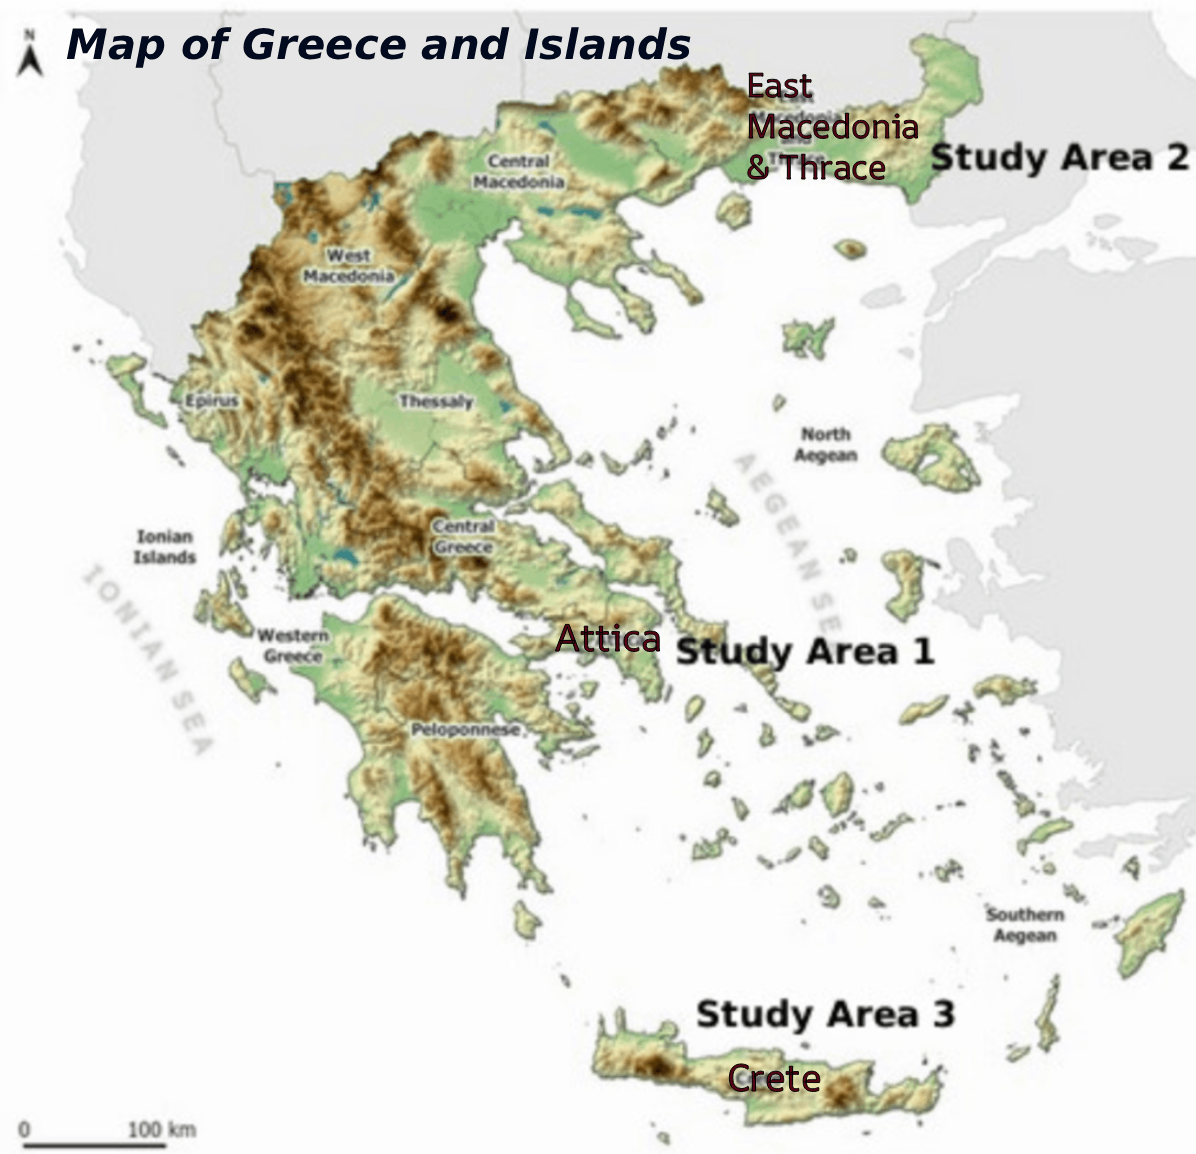
\includegraphics{Greece_map3}
\par\end{centering}
\caption{Map of Greece and Islands highlighting the three geographic study
areas (Study Area 1: Attica, Study Area 2: Eastern Macedonia \& Thrace,
Study Area 3: Crete).\label{fig:Map-with-areas}}
\end{figure}

The climatological and fire dataset for all regions cover the period
from 1 January 2000 to 31 December 2024. Specifically, Attica contains
9.131 climatological records and 2.736 fire records, Eastern Macedonia
and Thrace contains 9.131 climatological records and 10.358 fire records,
and Crete contains 9.121 climatological records and 6.036 fire record.
The slight variation in the number of climatological records is attributable
to missing values in the data retrieved from Visual Crossing, and
did not affect the results of the analysis. 

\textbf{Regarding missing data in the Visual Crossing, the meteorological
dataset for Attica contained 9.131 daily records (2000--2024), and
the dataset for Eastern Macedonia \& Thrace contained the same number
of records for the same period. The dataset for Crete exhibited a
small gap of 10 missing daily records during May 18--28, 2001. This
gap does not affect the merged dataset or the class construction procedure,
because during that specific period only two wildfire incidents occurred,
both of which were short duration events and were not included in
the analysis. Therefore, the missing data do not influence the threshold
derivation, the class definitions, or the subsequent machine learning
experiments.}

Before proceeding with the merging of the two data files, the experiments
focused exclusively on forest fire incidents in order to maintain
homogeneity in our dataset with respect to fire behavior characteristics.
In other words, we chose to proceed with the following categories
: (9) Burned forests, (10) Burned forest area, and (11) Burned grove
(small forest) Table \ref{tab3:Table_3_Primary-table-with}. Following
this refinement, Attica provided 1.859 forest fire records, Eastern
Macedonia and Thrace 2.653, and Crete 2.789.

Afterwards, the climatological dataset merged with the forest fire
dataset, retaining only the climate records corresponding to the fire
ignition date. The merging process was performed combining the climatological
data from Table \ref{tab2:Table_2Primary-table-with} with the fire
incident data from Table \ref{tab3:Table_3_Primary-table-with} based
on the date field. 

\begin{table}[H]
\centering
\caption{Primary table of raw climatological variables (33 attributes) retrieved
from the Visual Crossing platform for the period 2000--2024.\label{tab2:Table_2Primary-table-with}}

\begin{tabular*}{14cm}{@{\extracolsep{\fill}}|c|c|c|}
\hline 
\textbf{Number} & \textbf{Data Description} & \textbf{Values}\tabularnewline
\hline 
\hline 
1 & Region & Area\tabularnewline
\hline 
2 & Date & Year/month/day\tabularnewline
\hline 
3 & Temp max (Fahrenheit) & \textdegree F\tabularnewline
\hline 
4 & Temp min (Fahrenheit) & \textdegree F\tabularnewline
\hline 
5 & Temp (Fahrenheit) daily mean average & \textdegree F\tabularnewline
\hline 
6 & Feels like max (Fahrenheit) & \textdegree F\tabularnewline
\hline 
7 & Feels like min (Fahrenheit) & \textdegree F\tabularnewline
\hline 
8 & Feels like (Fahrenheit) & \textdegree F\tabularnewline
\hline 
9 & Dew & \textdegree F\tabularnewline
\hline 
10 & Humidity & \%\tabularnewline
\hline 
11 & Precipitation & in\tabularnewline
\hline 
12 & Precip prob & \%\tabularnewline
\hline 
13 & Precip cover & \%\tabularnewline
\hline 
14 & Precip type & Type(s)\tabularnewline
\hline 
15 & Snow & in\tabularnewline
\hline 
16 & Snow depth & in\tabularnewline
\hline 
17 & Windgust (miles) & mph\tabularnewline
\hline 
18 & Windspeed (miles) & mph\tabularnewline
\hline 
19 & Wind dir & (\textdegree)\tabularnewline
\hline 
20 & Sea level & mb\tabularnewline
\hline 
21 & Cloud cover & \%\tabularnewline
\hline 
22 & Visibility & mi\tabularnewline
\hline 
23 & Solar radiation & (W/m\texttwosuperior )\tabularnewline
\hline 
24 & Solar energy & (MJ/m\texttwosuperior )\tabularnewline
\hline 
25 & Uvindex & (0-10)\tabularnewline
\hline 
26 & Severisk & (0-100)\tabularnewline
\hline 
27 & Sunrise & time\tabularnewline
\hline 
28 & Sunset & time\tabularnewline
\hline 
29 & Moon phase & (0-1)\tabularnewline
\hline 
30 & Conditions & general observations\tabularnewline
\hline 
31 & Descriptions & general observations day/night\tabularnewline
\hline 
32 & Icon & summarized observations\tabularnewline
\hline 
33 & Stations & Code for stations\tabularnewline
\hline 
\end{tabular*}
\end{table}

\begin{table}[H]
\centering
\caption{Primary table of raw operational forest fire incident data (16 attributes)
as recorded by the Hellenic Fire Service.\label{tab3:Table_3_Primary-table-with}}

\begin{tabular*}{10cm}{@{\extracolsep{\fill}}|c|c|}
\hline 
\textbf{Number} & \textbf{Data Description}\tabularnewline
\hline 
\hline 
1 & Fire department\tabularnewline
\hline 
2 & Forest department\tabularnewline
\hline 
3 & Location\tabularnewline
\hline 
4 & Region\tabularnewline
\hline 
5 & Date of fire ignition\tabularnewline
\hline 
6 & Time of fire ignition\tabularnewline
\hline 
7 & Extinguish date\tabularnewline
\hline 
8 & Extinguish time\tabularnewline
\hline 
9 & Burned forests\tabularnewline
\hline 
10 & Burned forests area\tabularnewline
\hline 
11 & Burned grove (small forest)\tabularnewline
\hline 
12 & Burned grassland\tabularnewline
\hline 
13 & Burned swamps\tabularnewline
\hline 
14 & Burned agricultural\tabularnewline
\hline 
15 & Burned crops\tabularnewline
\hline 
16 & Burned garbage dumps\tabularnewline
\hline 
\end{tabular*}
\end{table}

Accordingly, we created three new datasets, one for each study region.
Each region was examined and analyzed independently, resulting in
a distinct fire risk classification for every area. Consequently,
the variables processed in order to construct the class representing
danger forest fire ignition, for all three datasets were the following:
mean daily temperature, daily humidity values, precipitation occurrence,
wind gusts, wind speed, wind direction, time of fire ignition, month
of fire ignition, and fire duration, with the final output expressed
as the Final\_DangerClass\_combination Table \ref{tab4:Table_4_Modified-Data}.
In the end, in order to ensure impartiality in our experiments, we
removed the Fire Duration feature \citep{Kopitsa 2024}, since the
model would otherwise be able to see the answer, as the accuracy for
all datasets reached 100\%. 

\begin{table}[H]
\centering
\caption{Final derived variables/classes obtained after processing the raw
data, used to construct the target variable Final\_DangerClass\_combination.\label{tab4:Table_4_Modified-Data}}

\begin{tabular*}{10cm}{@{\extracolsep{\fill}}|c|c|}
\hline 
\textbf{Number} & \textbf{Data}\tabularnewline
\hline 
\hline 
1 & Temp Special Class (daily mean average)\tabularnewline
\hline 
2 & Humidity Special Class\tabularnewline
\hline 
3 & Precipitation Basic Class\tabularnewline
\hline 
4 & Windgust Special Class\tabularnewline
\hline 
5 & Windspeed Special Class\tabularnewline
\hline 
6 & Wind dir Special Class\tabularnewline
\hline 
7 & Time Class\tabularnewline
\hline 
8 & Month class\tabularnewline
\hline 
9 & Fire duration (Removed)\tabularnewline
\hline 
10 & Final\_DangerClass\_combination\tabularnewline
\hline 
\end{tabular*}
\end{table}


\subsubsection{\textit{Construction of region-specific fire-danger thresholds and
classes. }}

\textbf{To identify the thresholds of the climatological features
associated with long-duration wildfire / forest-fire events, the following
procedure was applied independently to each region and its corresponding
dataset. }

\textbf{The first step involved defining the critical duration threshold
for long-duration forest fires. In the Greek context, this threshold
is set at 360 minutes\citep{Kopitsa 2024}, since if a wildfire is
not brought under control within the first few hours, it tends to
spread rapidly beyond containment and may continue burning for several
days \citep{Kopitsa 2025}. Accordingly, wildfires with a duration
of up to 360 minutes, were assigned to (class\,0), whereas wildfires
with a duration of 361 minutes or more were assigned assigned to the
long duration, (class 1). }

\textbf{Subsequently, a systematic data-driven procedure, based on
statistical mean estimation and iterative refinement, was applied
to determine the hazardous values for each feature, as in Table \ref{tab4:Table_4_Modified-Data}.
Specifically, the mean value of each climatological variable was first
computed. Each initial cutoff was then evaluated by filtering the
data according to the fire-duration attribute, in order to assess
its ability to distinguish long-duration (class 1) from short-duration
fires (class 0). }

\textbf{For example, in the Attica dataset, the mean temperature observed
during wildfire events was 74.80}\textdegree\textbf{F. Accordingly,
an initial classification rule was applied whereby temperatures up
to 74.80}\textdegree\textbf{F were assigned to class\,0, while temperatures
of 74.81}\textdegree\textbf{F and above were assigned to class\,1.
This preliminary cutoff was then evaluated against the fire-duration
feature to assess the extent to which class\,1 values corresponded
to long-duration fires. In this case, inconsistencies were identified,
and the threshold refinement procedure was continued. Through this
process, the final temperature threshold for Attica was determined
to be 73.7}\textdegree\textbf{F. }

\textbf{An analogous refinement procedure was applied to all remaining
climatological variables and across all regional datasets, yielding
the final set of hazardous and non hazardous thresholds presented
in Tables\,\ref{tab5:Table_5_Modified_Special_-Classes}, \ref{tab6:Modified_Special_-Classes_EastMa}, and \ref{tab7:Table_7_Modified_Special_-Classes_Crete}. }

\textbf{In summary, this study followed a data\nobreakdash-driven
to identify hazardous climatological values rather than relying on
a traditional climatological analysis. Meteorological data and operational
fire-incident records were merged for the same time period. Long-
duration wildfires were then filtered, and the relevant variables
temperature, humidity, precipitation probability, wind speed, wind
gusts, wind direction, ignition time, and month, were isolated. New
empirical hazard thresholds associated with long-duration wildfire
events were subsequently computed.}

\textbf{Based on these values, binary classes (0/1) were defined for
each feature, where 1 denotes a hazardous value and 0 a non- hazardous
value. Subsequently, a new dataset was constructed containing the
transformed feature columns and the corresponding final danger class,
and a ten - fold cross validation procedure was applied to evaluate
the experimental results.}

\textbf{Thus, a regionally adapted forest-fire danger index was developed
based on real climatological and operational data. Unlike the uniform
30/30/30 rule, the proposed index uses thresholds and weights tailored
to the specific characteristics of each region. Since, the final danger
class is derived from the transformed input variables, the classification
experiments are interpreted as assessing the reproducibility of the
proposed rule, with independent operational validation remains necessary. }

\subsubsection{\textit{Impacts and consequences of forest-fire disasters.}}

\textbf{We next provide a concise overview of the consequences and
broader impacts associated with wildfires / forest-fires. To begin
with, wildfires substantially elevate air pollution levels. According
to the World Health Organization, wildfire smoke constitutes a major
source of toxic gaseous and particulate pollutants, as well as an
important contributor to greenhouse gas emissions \citep{WHO 2026}.
In the Figure \ref{fig:Chart-of-carbon}, the carbon dioxide emissions
(in tons) released into the atmosphere from wildfires in Greece during
the period 2003--2025 are shown, as estimated by the Global Wildfire
Information System. }

\begin{figure}[H]
\centering
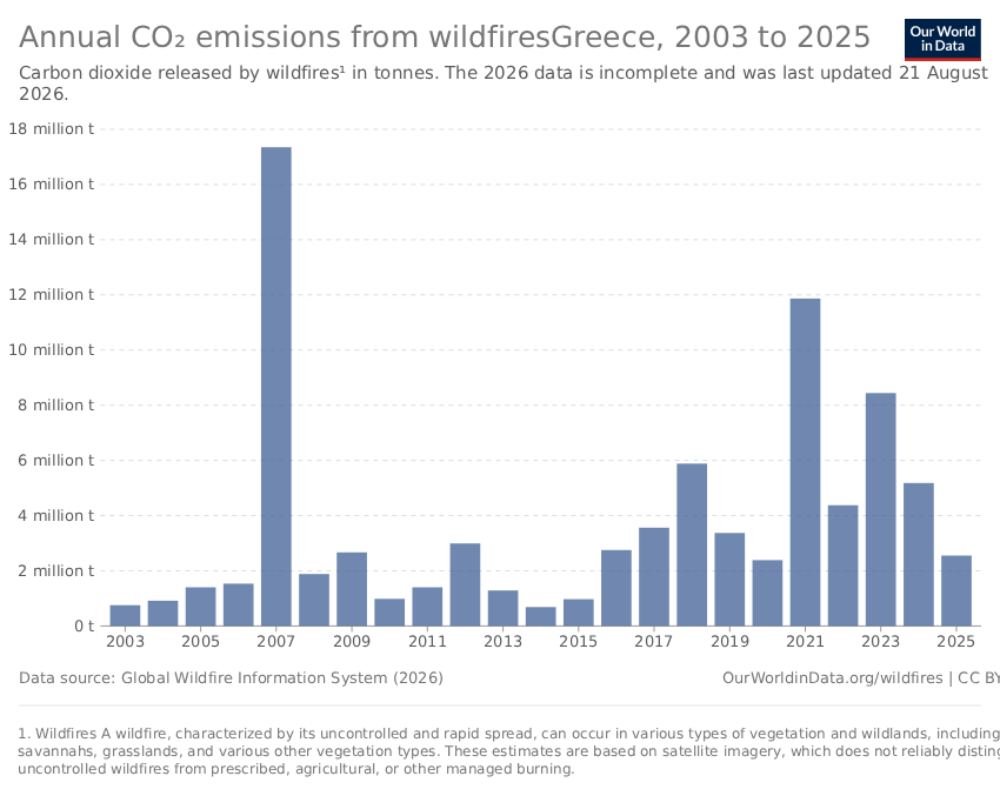
\includegraphics{annual-carbon-dioxide-emissions(6)}

\caption{Chart of carbon emissions from wildfires in Greece during the period
2003--2025\label{fig:Chart-of-carbon}.}

\end{figure}

\textbf{In addition to air pollution, wildfires also affect a country’s
economic stability, as illustrated in the Figure \ref{fig:Chart-of-economic}.
The chart illustrates economic losses from disasters as a percentage
of gross domestic product (GDP), with wildfire related damages shown
in orange. }

\begin{figure}[H]
\centering
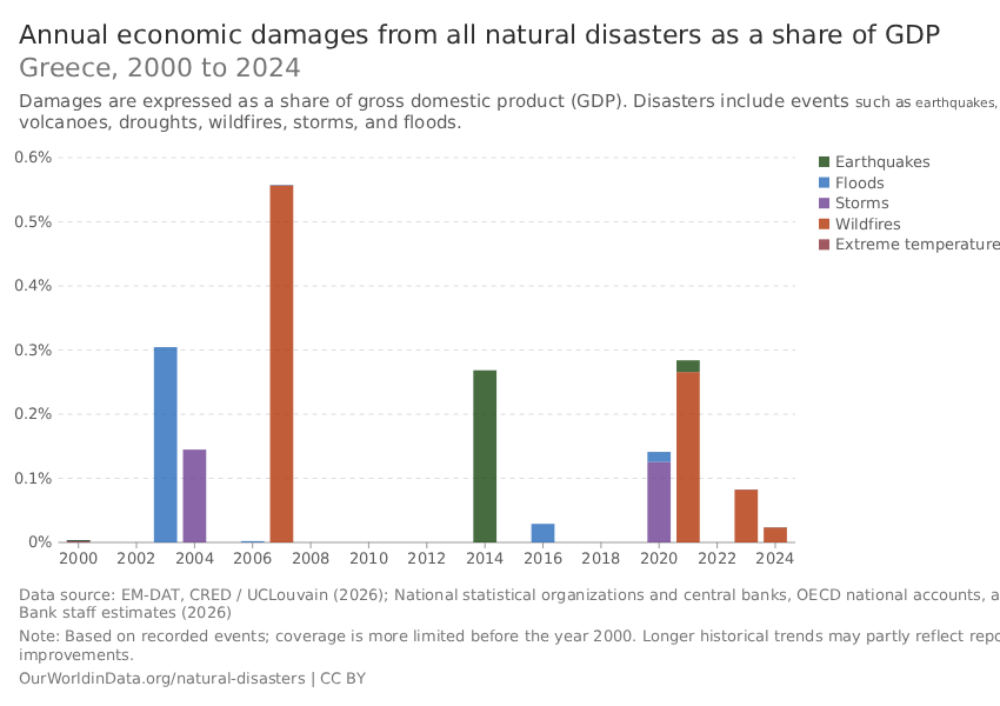
\includegraphics{natural-disasters-economic-damages}

\caption{Chart of economic damages from all natural disasters during the period
2000 - 2025\label{fig:Chart-of-economic}}

\end{figure}

\textbf{In parallel, the number of people affected by a wildfire often
reaches into the thousands, including individuals sustaining physical
injuries, those requiring immediate assistance, and people left homeless
who need temporary shelter because their homes were destroyed or severely
damaged during the disaster, Figure \ref{fig:Chart-of-people}.}

\begin{figure}[H]
\centering

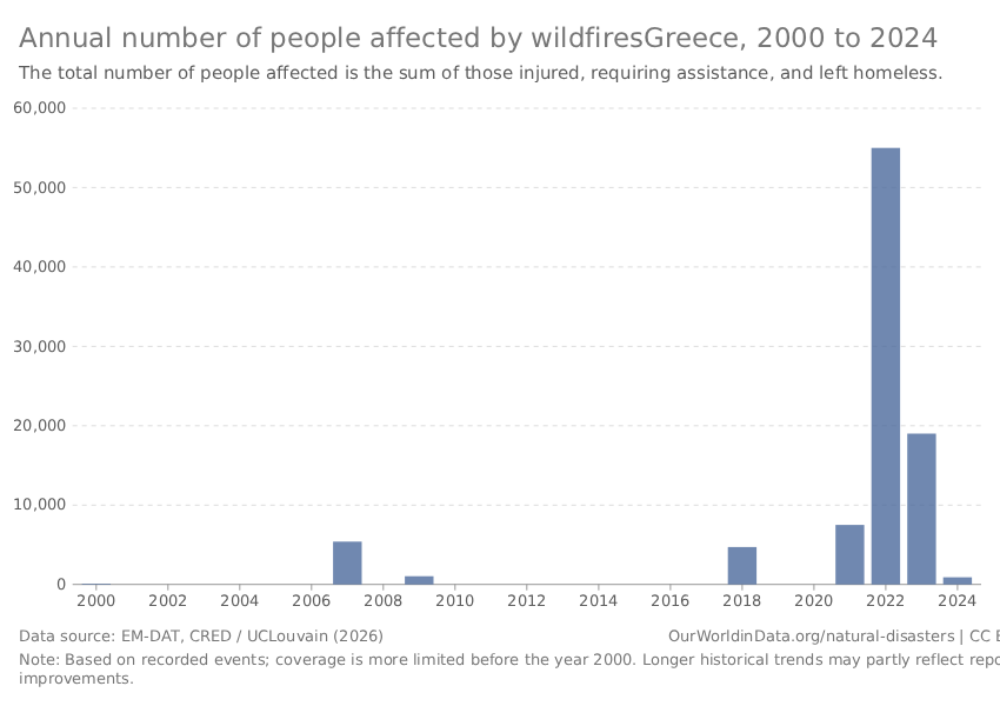
\includegraphics{natural-disasters-people-affected}

\caption{Chart of people affected from forest fires during the period 2000
- 2024\label{fig:Chart-of-people}}

\end{figure}

\textbf{In closing, when discussing the impacts of wildfires, it is
essential to acknowledge the loss of human life, the most severe and
irreversible of all consequences, Figure \ref{fig:Chart-of-annual}.
In summary, reducing the societal and environmental impacts of wildfires
brings to the forefront the need for precise, region specific definitions
of climatological thresholds that favor the development of long-duration
wildfire events.}

\begin{figure}[H]
\centering

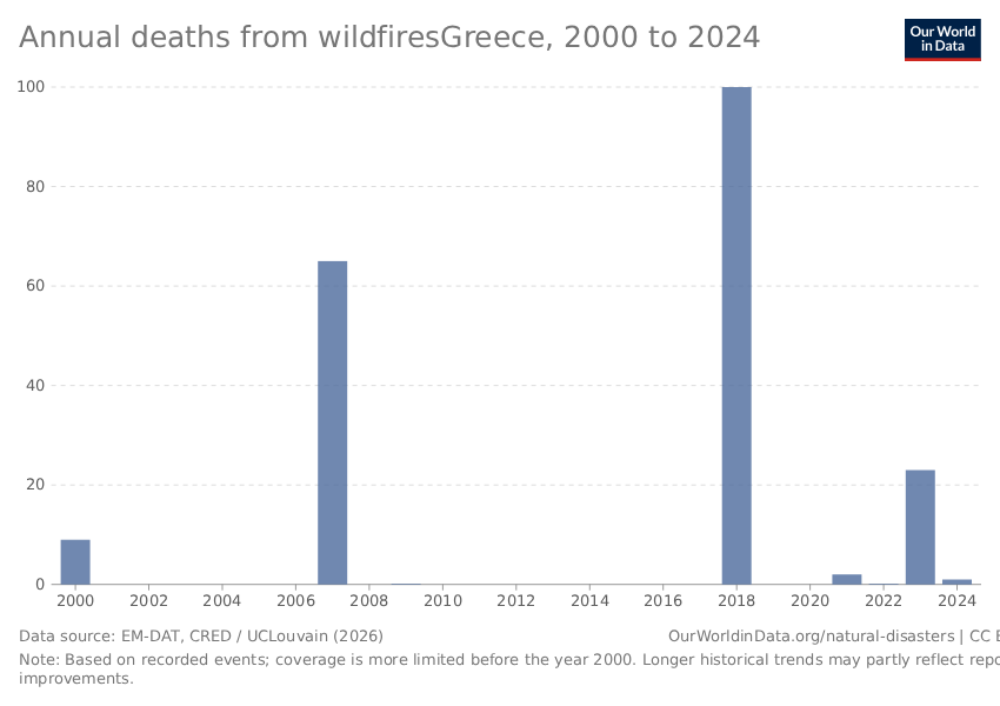
\includegraphics{natural-disasters-deaths}

\caption{Chart of annual deaths from forest fires during the period 2000 -
2024\label{fig:Chart-of-annual}}

\end{figure}

\textbf{Next, we describe the data used for each region separately. }

\subsubsection{\textit{Attica area and data description}}

The regional unit of Attica covers an area of 3,808.1\,km\texttwosuperior ,
with Athens as its capital. Between 2001 and 2025, Attica experienced
a loss of 22\,kha (220 km\texttwosuperior ) of tree cover attributable
to wildfires, along with an additional 3.3\,kha (33 km\texttwosuperior )
lost due to other disturbance factors. The most severe year within
this period was 2021, during which fires accounted for 8.5\,kha (85
km\texttwosuperior ) of tree cover loss, representing 99\% of the
total loss recorded that year, according to the global forest watch
\citep{Global Forest Watch Attica}. 

A brief description of the Attica dataset follows. The final dataset
consisted of 1.859 records and 8 attributes, with the last attribute
representing the target class, namely: Final\_DangerClass\_combination.
The classes followed a binary scheme, where 0 denoted a non hazardous
value, and 1 denoted as a hazardous value, in the following Table
\ref{tab5:Table_5_Modified_Special_-Classes}. 

\begin{table}[H]
\caption{Definition of the threshold values (temperature, humidity, wind, wind
direction, ignition time, month) separating the non-hazardous (Class
0) from the hazardous (Class 1) fire danger class for the Attica region,
with the corresponding number of records per class.\label{tab5:Table_5_Modified_Special_-Classes}}

\centering{}%
\begin{tabular}{|c|c|c|}
\hline 
\textbf{Features} & \textbf{Class 0 (non hazard)} & \textbf{Class 1 (hazard)}\tabularnewline
\hline 
\hline 
{\small Temp Special Class (daily mean average)} & \textless{} (73.6\textdegree F){\footnotesize{} (lower)} & \textgreater{} 73.7\textdegree F (or 23.6\textdegree C) {\footnotesize (higher)}\tabularnewline
\hline 
{\small Humidity Special Class} & \textgreater{} 49.4\% (higher) & \textless{} 49.3\% (lower)\tabularnewline
\hline 
{\small Precipitation Basic Class} & rain & no rain\tabularnewline
\hline 
{\small Windgust Special Class} & \textless{} 10miles (lower) & \textgreater{} 10.01miles (higher)\tabularnewline
\hline 
{\small Windspeed Special Class} & \textless{} 16miles (lower) & \textgreater{} 16.1miles (higher)\tabularnewline
\hline 
{\small Wind dir Special Class} & (S, SE, E, W) & (SW, N, NE, NW)\tabularnewline
\hline 
{\small Time Class} & \textless{} 12:30 (before) & \textgreater{} 12:31 (after)\tabularnewline
\hline 
{\small Month class} & (1,2,3,4,5,9,10,11,12) & (6,7,8{*})\tabularnewline
\hline 
{\small Final\_DangerClass\_combination} & 844 data & 1.015 data\tabularnewline
\hline 
\end{tabular}
\end{table}

In summary, the findings of the study identified new threshold values
for wildfire occurrence in the region of Attica, as follows: temperature
$\ge$ 73.7\,\textdegree F, humidity $\le$49.3\%, 0\% precipitation,
wind gust speed $\ge$10.01\,mph, wind speed $\ge$16.1\,mph, wind
direction in the sectors SW, N, NE, and NW, ignition time from 12:31
on wards, and hazardous months corresponding to June, July, and August{*}.

\subsubsection{Eastern Macedonia and Thrace area and data description}

The regional unit of Eastern Macedonia and Thrace, covers an area
of 14.158 km\texttwosuperior , with Komotini as its capital. Between
2001 to 2025, Eastern Macedonia and Thrace experienced a loss of 40
kha (400 km\texttwosuperior ) of tree cover attributable to wildfires,
along with an additional 11 kha (110 km\texttwosuperior ) lost due
to other disturbance factors. The most severe year within this period
was 2023, during which fires accounted for 31 kha (310 km\texttwosuperior )
of tree cover loss, representing 94\% of the total loss recorded that
year, according to the global forest watch\citep{Global Forest Watch Attica}. 

A brief description of the Eastern Macedonia and Thrace dataset follows.
The final dataset consisted of 2.653 records and 8 attributes, with
the last attribute representing the target class, namely: Final\_DangerClass\_combination.
The classes follow the same binary scheme as previously. A concise
summary table of these variables is presented in Table \ref{tab6:Modified_Special_-Classes_EastMa}. 

\begin{table}[H]
\caption{Definition of the threshold values (temperature, humidity, wind, wind
direction, ignition time, month) separating the non-hazardous (Class
0) from the hazardous (Class 1) fire danger class for the Eastern
Macedonia \& Thrace region, with the corresponding number of records
per class.\label{tab6:Modified_Special_-Classes_EastMa}}

\centering{}%
\begin{tabular}{|c|c|c|}
\hline 
\textbf{Features} & \textbf{Class 0 (non hazard)} & \textbf{Class 1 (hazard)}\tabularnewline
\hline 
\hline 
{\small Temp Special Class (daily mean average)} & \textless{} 68\textdegree F {\footnotesize (lower)} & \textgreater 68.1\textdegree F (or 20\textdegree C){\footnotesize{}
(higher)}\tabularnewline
\hline 
{\small Humidity Special Class} & \textgreater{} 64.1\% (higher) & \textless{} 64\% (lower)\tabularnewline
\hline 
{\small Precipitation Basic Class} & rain & no rain\tabularnewline
\hline 
{\small Windgust Special Class} & \textless{} 7miles (lower) & \textgreater{} 7.1miles (higher)\tabularnewline
\hline 
{\small Windspeed Special Class} & \textless{} 6miles (lower) & \textgreater{} 6.1miles (higher)\tabularnewline
\hline 
{\small Wind dir Special Class} & (W,NW,N) & (E,SE,SW,S,NE)\tabularnewline
\hline 
{\small Time Class} & \textless{} = 11:30 & 11:31 =\textgreater\tabularnewline
\hline 
{\small Month class} & (1,2,3,4,9,11,12) & (5,6,7,8,10{*})\tabularnewline
\hline 
{\small Final\_DangerClass\_combination} & 1.093 & 1.560\tabularnewline
\hline 
\end{tabular}
\end{table}

In summary, the findings of the study identified new threshold values
for wildfire occurrence in the region of Eastern Macedonia and Thrace,
as follows: temperature $\ge$ 68.1\,\textdegree F, humidity $\le$
64.1\%, 0\% precipitation, wind gust speed $\ge$ 7.1\,mph, wind speed
$\ge$ 6.1\,mph, wind direction in the sectors E, S, SW, SE, and NE,
ignition time from 11:31 on wards, and hazardous months corresponding
to May, June, July, August and October.

\subsubsection{\textit{Crete area and data description }}

The regional unit of Crete covers an area of 8.450 km\texttwosuperior ,
with Herakleio as its capital. Between 2001 to 2025 Crete experienced
a loss of 1.3 kha (13 km\texttwosuperior ) of tree cover attributable
to wildfires, along with an additional 3.2 kha (32 km\texttwosuperior )
lost due to other disturbance factors. The most severe year within
this period was 2008 during which fires accounted for 210 ha (2.1
km\texttwosuperior ) of tree cover loss, representing 44\%, of the
total loss recorded that year, according to the global forest watch
\citep{Global Forest Watch Attica}. 

A brief description of the Crete datasets follows in Table \ref{tab7:Table_7_Modified_Special_-Classes_Crete}. 

\begin{table}[H]
\caption{Definition of the threshold values (temperature, humidity, wind, wind
direction, ignition time, month) separating the non-hazardous (Class
0) from the hazardous (Class 1) fire danger class for the Crete region,
with the corresponding number of records per class.\label{tab7:Table_7_Modified_Special_-Classes_Crete}}

\centering{}%
\begin{tabular}{|c|c|c|}
\hline 
\textbf{Features} & \textbf{Class 0 (non hazard)} & \textbf{Class 1 (hazard)}\tabularnewline
\hline 
\hline 
{\small Temp Special Class (daily mean average)} & \textless{} 70\textdegree F{\footnotesize{} (lower)} & \textgreater 70.1\textdegree F (or 20.17\textdegree C){\footnotesize{}
(higher)}\tabularnewline
\hline 
{\small Humidity Special Class} & \textgreater{} 66.1\% (higher) & \textless{} 66\% (lower)\tabularnewline
\hline 
{\small Precipitation Basic Class} & rain & no rain\tabularnewline
\hline 
{\small Windgust Special Class} & \textless{} 9miles (lower) & \textgreater{} 9.1miles (higher)\tabularnewline
\hline 
{\small Windspeed Special Class} & \textless{} 16miles (lower) & \textgreater{} 16.1miles (higher)\tabularnewline
\hline 
{\small Wind dir Special Class} & (S, SW, SE, E, W) & (N, NE, NW)\tabularnewline
\hline 
{\small Time Class} & \textless{} = 12:30 & 12:31 =\textgreater\tabularnewline
\hline 
{\small Month class} & (1,2,3,4,5,9,10,11,12) & (6,7,8{*})\tabularnewline
\hline 
{\small Final\_DangerClass\_combination} & 1.384 & 1.405\tabularnewline
\hline 
\end{tabular}
\end{table}

In summary, the findings of the study identified new threshold values
for wildfire occurrence in the region of Crete, as follows: temperature
$\ge$ 70.1\,\textdegree F, humidity $\le$66\%, 0\% precipitation,
wind gust speed $\ge$9.1\,mph, wind speed$\ge$ 16.1\,mph, wind direction
in the sectors N, NE, and NW, ignition time from 12:31 on wards, and
hazardous months corresponding to June, July, and August .

\subsubsection{\textit{The feature construction method}}

\textbf{For a subset of the conducted experiments, a feature construction
technique \citep{fc1} involving two artificial features was employed.
A brief description of the applied procedure is provided below. This
method generates artificial features from the original input variables
through the Grammatical Evolution process. The resulting features
represent non-linear transformations of the initial features. In recent
years, this method has been applied to several real-world problems,
including earthquakes \citep{Tsoulos 2026}, flash flood \citep{Liu 2024},
fetal heart rate \citep{Georgoulas 2007}, spam recognition \citep{Gavrilis 2006}
etc. The extended version of BNF grammar used during the feature construction
process is outlined in Figure \ref{fig:The-extended-BNF}}

\begin{figure}[H]

\includegraphics{\string"BNF grammar\string".png}

\caption{The extended BNF grammar used in the feature construction process\label{fig:The-extended-BNF}}

\end{figure}

The main steps of the used algorithm are as follows:

\begin{doublespace}
\textbf{1. Initialization step.}

(a) \textbf{Define} the number of used chromosomes $N_{c}$.

(b) \textbf{Define} the maximum number of allowed generations $N_{g}$.

(c) \textbf{Set} the selection rate $p_{s}\in[0,1]$ and the mutation
rate $p_{m}\in[0,1]$.

(d) \textbf{Set} as $N_{f}$ the number of desired features that will
be created.

(e) \textbf{Set} $k=0$, the generation number.

2. \textbf{Fitness calculation step}.

3. \textbf{For $i=1,\ldots,N_{c}$ do}

(a) \textbf{Create} with the assistance of Grammatical Evolution,
a set of $N_{f}$ artificial features from the original ones, for
chromosome $g_{i}$.

(b) \textbf{Transform} the original train set using the previously
produced features. Represent the new set as $\mbox{TR}=\left(x_{g_{i},j},t_{j}\right),\ j=1,..M$

(c) \textbf{Apply }a machine learning model denoted as $C$ on set
TR and train this model and denote as $C(x)$ the output of this model
for any input pattern $x$.

(d) \textbf{Calculate} the fitness $f_{i}$ as:
\begin{equation}
f_{i}=\sum^{M}_{j=1}\left(C\left(x_{g_{i},j}\right)-t_{j}\right)^{2}
\end{equation}
The Radial Basis Function (RBF) networks \citep{Park 1991,Yu 2011}
were used as the machine learning models $C(x)$ in the current work.
This machine learning model was chosen because of the significantly
shorter training time it requires compared to other machine learning
models. 

4. \textbf{End For}

5. \textbf{Genetic operations step. }Perform the same genetic operators
as in the case of construction neural networks, discussed previously.

6. \textbf{Termination check step}.

(a) \textbf{Set} $k=k+1$ 

(b) \textbf{If} $k\le N_{g}$ then go to Fitness Calculation Step.

7. \textbf{Application to the test set}.

(a) \textbf{Obtain} the chromosome $g^{*}$ with the lowest fitness
value.

(b) \textbf{Create} the $N_{f}$ artificial features that correspond
to this chromosome

(c) \textbf{Apply} the $N_{f}$ features to the train set and produce
the mapped training set $\mbox{TR}=\left(x_{g_{i},j},t_{j}\right),\ j=1,..M$

(d) \textbf{Train} a machine learning model on the produced training
set. An artificial neural network \citep{Bishop 1995,Cybenko 1989}
with $H=10$ processing nodes is used in the current work. This neural
network was trained using a BFGS variant of Powell \citep{powell}. 

(e) \textbf{Apply} the new features to the test set of the objective
problem and create the set $\mbox{TT=}\left(x_{g_{i},j},t_{j}\right),\ j=1,..K$

(f) \textbf{Apply} the machine learning model on set TT and report
the test error. 
\end{doublespace}

\section{Results\label{sec:Results}}

For the purposes of our experiments, we employed the available optimization
package Optimus\citep{Optimus}, which can be downloaded from\url{https://github.com/itsoulos/GlobalOptimus}
(accessed on 20 June 2026). For the feature construction process used
in the FC2 (RF) and FC2 (MLP) algorithms, we utilized the freely available
programming tool QFc\citep{QFC}, accessible at \url{https://github.com/itsoulos/QFc}
(accessed on 20 June 2026). In addition, the GENCLASS \citep{GenClass 2021}
system was employed in our experiments. GENCLASS is a free software
framework entirely written in ANSI C++, available by \url{https://github.com/itsoulos/GenClass/}(accessed
on 20 June 2026) designed to construct classification programs in
a C like programming language for the purpose of classifying input
data. It operates as an evolutionary rule induction method, generating
interpretable decision rules through genetic search mechanisms.

Each experiment was executed 30 times, using different seeds for the
random number generator in every run.\textbf{ For each experiment,
a complete ten - fold cross - validation procedure was performed,
resulting in 30 \texttimes{} 10 train-test evaluations for each algorithm
and dataset.} The proposed feature construction method was applied
independently to each fold, and the average classification errors
on the corresponding test sets were computed. For the experimental
tables the following notation was used:
\begin{enumerate}
\item The column DATASET denotes the dataset corresponding to a regions
where the machine learning methods were applied. Attica contains 1.859
records, of which 844 correspond to class 0 and 1.015 to class 1.
Eastern Macedonia \& Thrace contains 2.653 records, of which 1.093
correspond to class 0 and 1.560 to class 1. Crete contains 2.789 records,
of which 1.384 correspond to class 0 and 1.409 to class 1. 
\item The column MLP (BFGS) represents the application of an artificial
neural network \citep{nn1,nn2} with 10 processing nodes trained with
the BFGS optimization method \citep{powell}.
\item The column RBF stands for the usage of a Radial Basis Function (RBF)
network \citep{rbf1,rbf2} with 10 processing nodes.
\item The column RF denotes the application of the Random Forest model \citep{random_forest}.
\item The column FC2 (RF) represents the construction of two artificial
features using the Grammatical Evolution feature construction technique
\citep{fc1}. The Radial Basis Function (RBF) machine learning model
was employed for feature construction, while the generated features
were evaluated using Random Forests.
\item The column FC2 (MLP) stands for the construction of two artificial
features using the same feature construction technique. The evaluation
of the constructed features was performed using a neural network trained
with the BFGS method.
\item The column GENCLASS represents the incorporation of the GENCLASS method
to produce classification rules. 
\item The row AVERAGE represents the average classification error for each
dataset and method.
\end{enumerate}

\subsection{Classification error}

The results demonstrated in Table \ref{tab:Experimental-results-using}
that the model GENCLASS achieved the lower error accuracy in predicting
the final danger class, indicating that the newly developed fire danger
rule is fully identifiable and predictable based on the combined climatological
and operational fire incident data. 

\begin{table}[H]
\caption{Experimental results using the machine learning methods on various
regions. The numbers in cells represent average classification error.\label{tab:Experimental-results-using}}

\centering{}{\footnotesize{}%
\begin{tabular}{|c|c|c|c|c|c|c|}
\hline 
{\footnotesize DATASET} & {\footnotesize MLP (BFGS)} & {\footnotesize RBF} & {\footnotesize RF} & {\footnotesize FC2 (RF)} & {\footnotesize FC2 (MLP)} & {\footnotesize GENCLASS}\tabularnewline
\hline 
\hline 
{\footnotesize Attica} & {\footnotesize 13.67\%} & {\footnotesize 14.42\%} & {\footnotesize 13.93\%} & {\footnotesize 13.01\%} & {\footnotesize 12.82\%} & {\footnotesize 12.43\%}\tabularnewline
\hline 
\begin{cellvarwidth}[t]
\centering
{\footnotesize Eastern Macedonia }{\footnotesize\par}

{\footnotesize\& Thrace}
\end{cellvarwidth} & {\footnotesize 12.51\%} & {\footnotesize 15.34\%} & {\footnotesize 12.21\%} & {\footnotesize 11.93\%} & {\footnotesize 11.87\%} & {\footnotesize 11.47\%}\tabularnewline
\hline 
{\footnotesize Crete} & {\footnotesize 16.39\%} & {\footnotesize 17.82\%} & {\footnotesize 15.96\%} & {\footnotesize 16.15\%} & {\footnotesize 15.56\%} & {\footnotesize 14.86\%}\tabularnewline
\hline 
{\footnotesize\textbf{AVERAGE}} & {\footnotesize\textbf{14.19\%}} & {\footnotesize\textbf{15.86\%}} & {\footnotesize\textbf{14.03\%}} & {\footnotesize\textbf{13.70\%}} & {\footnotesize\textbf{13.42\%}} & {\footnotesize\textbf{12.92\%}}\tabularnewline
\hline 
\end{tabular}}{\footnotesize\par}
\end{table}

\begin{figure}[H]
\begin{centering}

\includegraphics[scale=0.6]{statistical_analysis_figure}
\par\end{centering}
\caption{Average classification error by , across the three study regions\label{fig:statClassification}}
\end{figure}

Figure \ref{fig:statClassification} presents, in bar-chart form,
the mean classification error rate (\%) achieved by each of the six
evaluated machine learning models, averaged across the three study
regions (Attica, Eastern Macedonia \& Thrace, and Crete), with error
bars representing one standard deviation. GENCLASS is visually distinguished
from the remaining five models and serves as the reference model against
which pairwise comparisons are drawn. It attained the lowest mean
classification error (12.92\%), followed in ascending order by FC2
(MLP) (13.42\%), FC2 (RF) (13.70\%), RF (14.03\%), MLP (BFGS) (14.19\%),
and RBF (15.86\%), the latter exhibiting both the highest mean error
and the greatest variability across regions. The figure further reports
the result of a Friedman test ($\chi^{2}$ = 14.05, df = 5, p = 0.015),
a non-parametric procedure appropriate for comparing multiple related
samples, which indicates that the observed differences in performance
among the six models are unlikely to have arisen by chance. Significance
markers displayed above each bar correspond to paired t-test comparisons
against GENCLASS: all models differ significantly from GENCLASS (p
\textless{} 0.05) with the exception of FC2 (RF), which is marked
as not significant (n.s.), suggesting that its performance is statistically
comparable to that of GENCLASS despite its marginally higher mean
error.

\begin{table}[H]
\caption{Statistical comparison of classification error, average ranking, and
significance tests (Wilcoxon and paired t-test) for the six machine
learning models relative to GENCLASS as the reference model.\label{tab:statClassification}}

\begin{centering}
\begin{tabular}{|c|c|c|c|c|c|c|c|c|c|}
\hline 
{\scriptsize Model} & \begin{cellvarwidth}[t]
\centering
{\scriptsize Mean}{\scriptsize\par}

{\scriptsize Error}
\end{cellvarwidth} & \begin{cellvarwidth}[t]
\centering
{\scriptsize SD}{\scriptsize\par}

{\scriptsize Error}
\end{cellvarwidth} & \begin{cellvarwidth}[t]
\centering
{\scriptsize Min }{\scriptsize\par}

{\scriptsize Error}
\end{cellvarwidth} & \begin{cellvarwidth}[t]
\centering
{\scriptsize Max}{\scriptsize\par}

{\scriptsize Error}
\end{cellvarwidth} & \begin{cellvarwidth}[t]
\centering
{\scriptsize Avg}{\scriptsize\par}

{\scriptsize Rank}
\end{cellvarwidth} & \begin{cellvarwidth}[t]
\centering
{\scriptsize Mean Diff vs }{\scriptsize\par}

{\scriptsize GENCLASS}
\end{cellvarwidth} & \begin{cellvarwidth}[t]
\centering
{\scriptsize Wilcoxon}{\scriptsize\par}

{\scriptsize p}
\end{cellvarwidth} & \begin{cellvarwidth}[t]
\centering
{\scriptsize Paired}{\scriptsize\par}

{\scriptsize p}
\end{cellvarwidth} & {\scriptsize Significance}\tabularnewline
\hline 
\hline 
{\scriptsize GENCLASS} & {\scriptsize 12.92} & {\scriptsize 1.75} & {\scriptsize 11.47} & {\scriptsize 14.86} & {\scriptsize 1} & {\scriptsize 0} &  &  & {\scriptsize Reference}\tabularnewline
\hline 
{\scriptsize FC2(MLP)} & {\scriptsize 13.42} & {\scriptsize 1.92} & {\scriptsize 11.87} & {\scriptsize 15.56} & {\scriptsize 2} & {\scriptsize -0.5} & {\scriptsize 0.1814} & {\scriptsize 0.0395} & {\scriptsize{*}}\tabularnewline
\hline 
{\scriptsize FC2(RF)} & {\scriptsize 13.7} & {\scriptsize 2.19} & {\scriptsize 11.93} & {\scriptsize 16.15} & {\scriptsize 3.33} & {\scriptsize -0.78} & {\scriptsize 0.1814} & {\scriptsize 0.0955} & {\scriptsize n.s.}\tabularnewline
\hline 
{\scriptsize RF} & {\scriptsize 14.03} & {\scriptsize 1.88} & {\scriptsize 12.21} & {\scriptsize 15.96} & {\scriptsize 4} & {\scriptsize -1.11} & {\scriptsize 0.1814} & {\scriptsize 0.0367} & {\scriptsize{*}}\tabularnewline
\hline 
{\scriptsize MLP(BFGS)} & {\scriptsize 14.19} & {\scriptsize 1.99} & {\scriptsize 12.51} & {\scriptsize 16.39} & {\scriptsize 4.67} & {\scriptsize -1.27} & {\scriptsize 0.1814} & {\scriptsize 0.0123} & {\scriptsize{*}}\tabularnewline
\hline 
{\scriptsize RBF} & {\scriptsize 15.86} & {\scriptsize 1.76} & {\scriptsize 14.42} & {\scriptsize 17.82} & {\scriptsize 6} & {\scriptsize -2.94} & {\scriptsize 0.1814} & {\scriptsize 0.0324} & {\scriptsize{*}}\tabularnewline
\hline 
\end{tabular}
\par\end{centering}
\end{table}

{\footnotesize\textit{Friedman test: chi-squared = 14.048, df = 5,
p-value = 0.0153}}{\footnotesize\par}

{\footnotesize\textit{Nemenyi critical difference (alpha = 0.05):
4.353}}{\footnotesize\par}

{\footnotesize\textit{Significance vs. GENCLASS (paired t-test): {*}{*}{*}
p\textless 0.001, {*}{*} p\textless 0.01, {*} p\textless 0.05,
n.s. = not significant}}{\footnotesize\par}

{\footnotesize\textit{Note: n = 3 regions per technique; results are
indicative given the small sample size.\medskip{}
}}{\footnotesize\par}

Table \ref{tab:statClassification} complements Figure \ref{fig:statClassification}
by providing a detailed statistical summary of model performance across
the three regions (n = 3 per model). For each model, the table reports
the mean, standard deviation, minimum, and maximum classification
error, together with the average rank obtained across regions, the
mean difference relative to GENCLASS, and the corresponding significance
estimates derived from both the Wilcoxon signed-rank test and the
paired t-test. GENCLASS consistently ranks first (average rank = 1)
with the lowest mean error and a comparatively narrow standard deviation
(SD = 1.75), whereas RBF ranks last (average rank = 6) with both the
highest mean error and the widest range of observed values. The Wilcoxon
test yields an identical p-value (0.1814) for all comparisons, which
is not statistically significant; this outcome reflects the limited
statistical power of the test given the very small sample size (n
= 3 paired observations per comparison). In contrast, the paired t-test,
being a parametric test with greater sensitivity under these conditions,
identifies statistically significant differences (p \textless{} 0.05)
between GENCLASS and all other models except FC2 (RF) (p = 0.0955,
n.s.), which again emerges as the closest competitor to GENCLASS.
The table footnote reports the overall Friedman test statistic ($\chi^{2}$
= 14.048, df = 5, p = 0.0153) and the Nemenyi critical difference
(4.353) used for post-hoc multiple comparisons, while explicitly cautioning
that, owing to the small sample size (three regions per technique),
the results should be regarded as indicative rather than conclusive.

Taken together, Figure \ref{fig:statClassification} and Table \ref{tab:statClassification}
converge on the conclusion that GENCLASS systematically outperforms
the remaining five models, with the superiority being statistically
robust, as confirmed by the paired t-test, against every model except
FC2 (RF), which stands out as its most competitive alternative.

\subsection{Precision and recall values}

Precision and recall are evaluation metrics used to assess the performance
of a machine learning model. Precision expresses the proportion of
predicted positive cases that are actually correct, while recall indicates
the proportion of true positive cases that the model successfully
identifies. Together, these metrics provide essential insight into
the effectiveness of a model in classification tasks. Precision is
calculated as: 
\begin{equation}
\mbox{Precision}=\frac{\mbox{True Positives}}{\mbox{True Positives}+\mbox{False Positives}}\label{eq:precision}
\end{equation}

Precision reflects the model’s ability to avoid false positives, making
it a key indicator of prediction reliability. In other words, the
higher the value, the fewer the errors. 

The Recall value confirms the model’s ability to correctly identify
the positive class, reflecting how many of the actual positive instances
were successfully detected. As with precision and recall, the higher
the value, the more successful the classification. Recall is calculated
as: 
\begin{equation}
\mbox{Recall}=\frac{\mbox{True Positives}}{\mbox{True Positives}+\mbox{False Negatives}}\label{eq:recall}
\end{equation}

The following table presents the average values of the precision and
recall measures for each dataset and for every method Table \ref{tab11:Precision-=000026-Recall}.
In this comparison as well, we observe the consistent performance
of all methods. The best values are achieved by RF, FC2 (RF), FC2
(MLP), and GENCLASS, while for the Eastern Macedonia \& Thrace dataset,
MLP (BFGS) stands out.

\begin{table}[H]
\caption{Comparative summary of average precision and recall values (\%) for
each machine learning technique, by study region (Attica, Eastern
Macedonia \& Thrace, Crete).\label{tab11:Precision-=000026-Recall}}

\centering{}%
\begin{tabular}{|c|c|c|c|c|c|c|c|}
\hline 
 &  & \multicolumn{1}{c|}{\begin{cellvarwidth}[t]
\centering
{\footnotesize MLP}{\footnotesize\par}

{\footnotesize (BFGS)}
\end{cellvarwidth}} & \multicolumn{1}{c|}{{\footnotesize RBF}} & \multicolumn{1}{c|}{{\footnotesize RF}} & \multicolumn{1}{c|}{\begin{cellvarwidth}[t]
\centering
{\footnotesize FC2}{\footnotesize\par}

{\footnotesize (RF)}
\end{cellvarwidth}} & \multicolumn{1}{c|}{\begin{cellvarwidth}[t]
\centering
{\footnotesize FC2}{\footnotesize\par}

{\footnotesize (MLP)}
\end{cellvarwidth}} & \multicolumn{1}{c|}{{\footnotesize GENCLASS}}\tabularnewline
\hline 
\hline 
\multirow{2}{*}{{\footnotesize Attica}} & {\footnotesize Precision} & {\footnotesize 87.98\%} & {\footnotesize 85.43\%} & {\footnotesize 88.07\%} & {\footnotesize 88.24\%} & {\footnotesize 88\%} & {\footnotesize\textbf{88.50\%}}\tabularnewline
\cline{2-8}
 & {\footnotesize Recall} & {\footnotesize 87.14\%} & {\footnotesize 85.32\%} & {\footnotesize 87.33\%} & {\footnotesize 87.32\%} & {\footnotesize 88.02\%} & {\footnotesize\textbf{88.10\%}}\tabularnewline
\hline 
\multirow{2}{*}{\begin{cellvarwidth}[t]
\centering
{\footnotesize Eastern}{\footnotesize\par}

{\footnotesize Macedonia}
\end{cellvarwidth}} & {\footnotesize Precision} & {\footnotesize 89.04\%} & {\footnotesize 83.51\%} & {\footnotesize\textbf{89.45\%}} & {\footnotesize 87.92\%} & {\footnotesize 88.08\%} & {\footnotesize 89\%}\tabularnewline
\cline{2-8}
 & {\footnotesize Recall} & {\footnotesize 88.05\%} & {\footnotesize 83.82\%} & {\footnotesize 88.37\%} & {\footnotesize 89.08\%} & {\footnotesize 89.08\%} & {\footnotesize\textbf{88.9\%}}\tabularnewline
\hline 
\multirow{2}{*}{{\footnotesize Crete}} & {\footnotesize Precision} & {\footnotesize 84.46\%} & {\footnotesize 82.09\%} & {\footnotesize 85.07\%} & {\footnotesize 84.95\%} & {\footnotesize 84.46\%} & {\footnotesize\textbf{85.07\%}}\tabularnewline
\cline{2-8}
 & {\footnotesize Recall} & {\footnotesize 84.39\%} & {\footnotesize 82.09\%} & {\footnotesize 85.03\%} & {\footnotesize 84.88\%} & {\footnotesize 84.52\%} & {\footnotesize\textbf{85.50\%}}\tabularnewline
\hline 
\end{tabular}
\end{table}

The precision and recall values presented in Table \ref{tab11:Precision-=000026-Recall}
confirm the pattern already observed for classification error, showing
consistently high and stable performance across all three regions.
For the Attica dataset, both metrics ranged between 85.32\% and 88.50\%,
with GENCLASS, FC2 (RF), and RF achieving the strongest results, while
RBF again recorded the lowest performance, at approximately 85\%.
The Eastern Macedonia \& Thrace dataset exhibited the highest overall
performance levels among the three regions, ranging from 83.51\% to
89.45\%, with RF, MLP (BFGS), and GENCLASS standing out in precision,
and FC2 (RF) and FC2 (MLP) achieving the highest recall values. In
contrast, the Crete dataset showed comparatively lower performance
levels, ranging from 82.09\% to 85.50\%, although the relative ranking
of the techniques remained consistent with the other two regions,
with GENCLASS and RF standing out. Across all three datasets, RBF
consistently underperformed relative to the other five techniques,
whereas GENCLASS, RF, and the feature construction methods FC2 (RF)
and FC2 (MLP) maintained the most stable and competitive precision
and recall values, corroborating the reliability of the region specific
fire danger thresholds developed in this study.

\begin{figure}[H]
\begin{centering}

\includegraphics[scale=0.6]{pr}
\par\end{centering}
\caption{Line chart of the average precision and recall (\%) across the three
study regions, for each machine learning model.\label{fig:precisionRacallChart}}

\end{figure}

Figure \ref{fig:precisionRacallChart} summarizes these findings,
showing that GENCLASS achieves the highest average recall across the
three regions (87.50\%) and an average precision (87.52\%) essentially
equivalent to that of RF, the top-performing model on this metric
(87.53\%), while RBF remains the weakest performing technique throughout.

\section{Conclusions\label{sec:Conclusions}}

This study developed and validated region specific fire danger classification
schemes for three climatically distinct areas of Greece, namely Attica,
Eastern Macedonia \& Thrace, and Crete, using twenty five years (2000-2024)
of combined climatological and operational fire incident data. Rather
than relying on the generic 30/30/30 rule, specialized threshold values
for temperature, humidity, wind gust, wind speed, wind direction,
ignition time, and month were derived independently for each region,
reflecting their distinct climatic profiles.\textbf{ Therefore, each
region was treated independently: the climatological and operational
data of Attica, Eastern Macedonia \& Thrace, and Crete were processed
separately, and the threshold construction (hazard class) procedure
was applied within each regional dataset. As a result, no cross -
region information leakage occurs. }

Six machine learning techniques were evaluated across all three datasets
using ten fold cross-validation: two classical approaches (MLP trained
with BFGS, and RBF networks), Random Forest (RF), two Grammatical
Evolution based feature construction methods (FC2 (RF) and FC2 (MLP)),
and GENCLASS, an evolutionary rule induction method also grounded
in Grammatical Evolution. The results consistently demonstrated a
clear performance hierarchy: GENCLASS achieved the lowest average
classification error (12.92\%) and the highest average precision and
recall values across all three regions, confirming that the fire danger
rule constructed in this study is \textbf{encouraging and emerges
directly} from climatological and operational data. FC2 (MLP) and
FC2 (RF) followed closely, ranking second and third respectively in
average classification error (13.42\% and 13.70\%), while the classical
techniques (RF, MLP (BFGS), and particularly RBF) exhibited comparatively
higher and more variable error rates, with RBF consistently ranking
last across all three regions in both classification error and precision/recall
metrics.

This pattern indicates that techniques grounded in Grammatical Evolution,
whether through automated feature construction (FC2) or direct rule
induction (GENCLASS), are better suited to capturing the complex,
region specific relationships between meteorological conditions and
wildfire occurrence than conventional neural network or ensemble based
approaches. In particular, the \textbf{strong performance} of GENCLASS
suggests that the interpretable decision rules it generates are not
only competitive in predictive accuracy but also offer a transparent
and operationally meaningful representation of fire danger, a property
that black box models such as MLP and RBF cannot provide. These findings
validate the climatological attributes and the region specific definitions
developed for the classification of fire danger, confirming that tailored,
evolutionarily derived thresholds provide a more reliable and robust
framework for wildfire risk assessment than generic, one size fits
all rules.

\textbf{However, it is crucial to acknowledge that these findings
are limited to the three regions examined in this study (Attica, Eastern
Macedonia \& Thrace, and Crete). The generalizability of the region-specific
classification schemes and the demonstrated superiority of Grammatical
Evolution-based methods cannot be assumed for other Greek regions
without external validation, particularly given the relatively small
effective sample size on which these conclusions are based. Thus,
while the results are encouraging for the examined areas, they represent
a promising but not yet fully generalizable framework that requires
validation across additional regions before broader operational deployment.}

Building on these findings, several directions merit further investigation.
First, the application of the proposed methodology to additional Greek
regions with different climatic and topographic characteristics would
help establish whether the observed \textbf{strong performance }of
Grammatical Evolution based techniques generalizes beyond the three
areas examined here. Second, incorporating additional predictive features,
such as vegetation type, fuel moisture content, terrain slope, and
proximity to human activity, could further improve the discriminative
power of the constructed classes, particularly for the Crete dataset,
which exhibited comparatively lower performance across all techniques.
Third, future work could explore the integration of the fire duration
variable, excluded in this study to preserve model impartiality, as
a secondary prediction target once ignition risk has been established,
thereby extending the framework from a binary danger classifier to
a more comprehensive operational decision support tool. Finally, given
the consistently strong performance of GENCLASS, further research
should focus on refining and extending the interpretability of the
generated rule sets, potentially enabling their direct adoption by
fire prevention services as a practical, region specific alternative
to the traditional 30/30/30 rule.

\vspace{6pt}


\authorcontributions{Conceptualization, C.K..; methodology, C.K.; software, I.G.T.; validation,
V.C.; formal analysis, V.C.; resources, G.K.; visualization, C.K.;
supervision, G.K. All authors have read and agreed to the published
version of the manuscript.}

\funding{This research has been financed by the European Union : Next Generation
EU through the Program Greece 2.0 National Recovery and Resilience
Plan , under the call RESEARCH -- CREATE -- INNOVATE, project name
“iCREW: Intelligent small craft simulator for advanced crew training
using Virtual Reality techniques\textquotedbl{} (project code:TAEDK-06195).}

\institutionalreview{Not applicable.}

\informedconsent{Not applicable.}

\dataavailability{The original contributions presented in this study are included in
the article. Further inquiries can be directed to the corresponding
author. }

\conflictsofinterest{The authors declare no conflicts of interest.}

\begin{adjustwidth}{-\extralength}{0cm}{}


\reftitle{References}
\begin{thebibliography}{99}
\bibitem{AA 2025} AA.com.tr. Southern California wildfires fully
contained after 24 days (2025). Available from: \url{https://www.aa.com.tr/en/americas/southern-california-wildfires-fully-contained-after-24-days/3468561}
(Last accessed on 01/05/2026). 

\bibitem{Bouvier 2025}Bouvier, V., Dedieu, K., Lyons, D., \& Raynaud,
R. (2025). When it burns in winter: Modelling off-season California
wildfires. Available from: \url{https://hal.science/hal-05240719/ }(Last
accessed on 01/05/2026). 

\bibitem{Visual crossing} Visual crossing.com. Available from: \url{https://www.visualcrossing.com/weather-query-builder/}
(Last accessed on 01/05/2026). 

\bibitem{NASA 2022}NASA. Wildfires Char South Korea. Available from:
\url{https://science.nasa.gov/earth/earth-observatory/wildfires-char-south-korea-149551/ }(Last
accessed on 01/05/2026). 

\bibitem{Weatherspark} WeatherSpark. Available from: \url{https://weatherspark.com/h/d/142033/2022/3/4/Historical-Weather-on-Friday-March-4-2022-in-Seoul-South-Korea}
(Last accessed on 01/05/2026). 

\bibitem{Modis Nasa 2025} Modis NASA. May 25, 2025 - Fires Continue
to Scorch Russia's Far East. Available from: \url{https://modis.gsfc.nasa.gov/gallery/individual.php?db_date=2025-05-25}
(Last accessed on 01/05/2026). 

\bibitem{WeatherSpark Russia} WeatherSpark. Available from: \url{https://weatherspark.com/d/127538/5/22/Average-Weather-on-May-22-in-Chita-Russia }(Last
accessed on 01/05/2026). 

\bibitem{Suzuki 2026} Suzuki, S., Manzello, S.L. The 2025 Wildland-Urban
Interface (WUI) Fire Disaster in Ofunato City, Japan. Fire Technol
62, 49 (2026). 

\bibitem{WeatherSpark japan} WeatherSpark. Available from: \url{https://weatherspark.com/d/144114/2/26/Average-Weather-on-February-26-in-\%C5\%8Cfunato-Japan}
(Last accessed on 01/05/2026). 

\bibitem{Cuevas 2021} Diaz Cuevas, M. D. P., \& Limones Rodriguez,
N. (2021). El papel de la regla 30/30/30 en los incendios forestales.
El caso de las provincias de Huelva y Sevilla. Available from: \url{https://idus.us.es/server/api/core/bitstreams/7c154de8-c760-442d-b95b-9b9d5a79944d/content }(Last
accessed on 12/05/2026). 

\bibitem{Cortez 2007} Cortez, P., \& Morais, A. D. J. R. (2007).
A data mining approach to predict forest fires using meteorological
data. New Trends in Artificial Intelligence, Proceedings of the 13th
EPIA, 512-523. 

\bibitem{Yunhao 2007} Yunhao, C., Jing, L., \& Guangxiong, P. (2007).
Forest fire risk assessment combining remote sensing and meteorological
information. New Zealand Journal of Agricultural Research, 50(5),
1037-1044. 

\bibitem{Sakr 2011}Sakr, G. E., Elhajj, I. H., \& Mitri, G. (2011).
Efficient forest fire occurrence prediction for developing countries
using two weather parameters. Engineering Applications of Artificial
Intelligence, 24(5), 888-894. 

\bibitem{Agarwal 2020}Agarwal, P., Tang, J., Narayanan, A. N. L.,
\& Zhuang, J. (2020). Big data and predictive analytics in fire risk
using weather data. Risk analysis, 40(7), 1438-1449. 

\bibitem{Masinda 2022} Masinda, M. M., Li, F., Qi, L., Sun, L., \&
Hu, T. (2022). Forest fire risk estimation in a typical temperate
forest in Northeastern China using the Canadian forest fire weather
index: case study in autumn 2019 and 2020. Natural hazards, 111(1),
1085-1101. 

\bibitem{Karali 2023} Karali, A., Varotsos, K. V., Giannakopoulos,
C., Nastos, P. P., \& Hatzaki, M. (2023). Seasonal fire danger forecasts
for supporting fire prevention management in an eastern Mediterranean
environment: the case of Attica, Greece. Natural hazards and earth
system sciences, 23(2), 429-445. 

\bibitem{Parvar 2024}Parvar, Z., Saeidi, S., \& Mirkarimi, S. (2024).
Integrating meteorological and geospatial data for forest fire risk
assessment. Journal of environmental management, 358, 120925. 

\bibitem{Kudl=0000E1=00010Dkov=0000E1 2025} Kudláčková, L., Bartošová,
L., Linda, R., Bláhová, M., Poděbradská, M., Fischer, M., ... \& Trnka,
M. (2025). Assessing fire danger classes and extreme thresholds of
the Canadian Fire Weather Index across global environmental zones:
a review. Environmental Research Letters, 20(1), 013001.

\bibitem{Hollis 2024} Hollis, J. J., Matthews, S., Anderson, W. R.,
Cruz, M. G., Fox-Hughes, P., Grootemaat, S., ... \& Sauvage, S. (2024).
A framework for defining fire danger to support fire management operations
in Australia. International Journal of Wildland Fire, 33(3), WF23141.

\bibitem{Grootemaat 2024} Grootemaat, S., Matthews, S., Kenny, B.
J., Runcie, J. W., Hollis, J. J., Sauvage, S., ... \& Holmes, A. (2024).
Live trial performance of the Australian fire danger rating system--research
prototype. International Journal of Wildland Fire, 33(4), WF23143

\bibitem{Barik 2026} Barik, A., \& Baidya Roy, S. (2026). FRAME v1.
0: Advancing Fire Risk Assessment in Tropical Fragmented Forests with
a Machine Learning Environment. EGUsphere, 2026, 1-24.

\bibitem{WHO 2026} World Health Organization. Wildfires, Wildfires
and air pollution. Available from: https://www.who.int/news-room/fact-sheets/detail/wildfires-and-health
(Last accessed on 23/08/2026). 

\bibitem{Global Forest Watch Attica} Global Forest Watch. Available
from: \url{https://www.globalforestwatch.org/dashboards/country/GRC/3/?category=fires&location=WyJjb3VudHJ5IiwiR1JDIiwiMyJd&map=eyJjYW5Cb3VuZCI6dHJ1ZX0\%3D}
(Last accessed on 02/05/2026). 

\bibitem{Tsoulos 2026} Kopitsa, C., Kyrou, G., Charilogis, V., \&
Tsoulos, I. G. (2026). Constructing Artificial Features with Grammatical
Evolution for Earthquake Prediction. Applied Sciences, 16(2), 746.

\bibitem{Liu 2024} Liu, Z., Felton, T., \& Mostafavi, A. (2024).
Interpretable machine learning for predicting urban flash flood hotspots
using intertwined land and built-environment features. Computers,
Environment and Urban Systems, 110, 102096.

\bibitem{Optimus} Tsoulos, I. G., Charilogis, V., Kyrou, G., Stavrou,
V. N., \& Tzallas, A. (2025). OPTIMUS: A Multidimensional Global Optimization
Package. Journal of Open Source Software, 10(108), 7584. 

\bibitem{Georgoulas 2007} Georgoulas, G., Gavrilis, D., Tsoulos,
I. G., Stylios, C., Bernardes, J., \& Groumpos, P. P. (2007). Novel
approach for fetal heart rate classification introducing grammatical
evolution. Biomedical Signal Processing and Control, 2(2), 69-79.

\bibitem{Gavrilis 2006} Gavrilis, D., Tsoulos, I. G., \& Dermatas,
E. (2006, May). Neural recognition and genetic features selection
for robust detection of e-mail spam. In Hellenic Conference on Artificial
Intelligence (pp. 498-501). Berlin, Heidelberg: Springer Berlin Heidelberg.

\bibitem{Park 1991} J. Park and I. W. Sandberg, Universal Approximation
Using Radial-Basis-Function Networks, Neural Computation 3, pp. 246-257,
1991.

\bibitem{Yu 2011} H. Yu, T. Xie, S. Paszczynski, B. M. Wilamowski,
Advantages of Radial Basis Function Networks for Dynamic System Design,
in IEEE Transactions on Industrial Electronics \textbf{58}, pp. 5438-5450,
2011.

\bibitem{Bishop 1995} C. Bishop, Neural Networks for Pattern Recognition,
Oxford University Press, 1995.

\bibitem{Cybenko 1989} G. Cybenko, Approximation by superpositions
of a sigmoidal function, Mathematics of Control Signals and Systems
\textbf{2}, pp. 303-314, 1989.

\bibitem{QFC} Tsoulos, I. G. (2022). QFC: A Parallel Software Tool
for Feature Construction, Based on Grammatical Evolution. Algorithms,
15(8), 295. 

\bibitem{GenClass 2021}Anastasopoulos, N., Tsoulos, I. G., \& Tzallas,
A. (2021). GenClass: A parallel tool for data classification based
on Grammatical Evolution. SoftwareX, 16, 100830.

\bibitem{Kopitsa 2024} Kopitsa, C., Tsoulos, I. G., Charilogis, V.,
\& Stavrakoudis, A. (2024). Predicting the duration of forest fires
using machine learning methods. Future Internet, 16(11), 396. 

\bibitem{Kopitsa 2025} Kopitsa C, Tsoulos IG, Miltiadous A, Charilogis
V. Predicting the Forest Fire Duration Enriched with Meteorological
Data Using Feature Construction Techniques. Symmetry. 2025; 17(11):1785.
https://doi.org/10.3390/sym17111785 

\bibitem{nn1}Müller, B., Reinhardt, J., \& Strickland, M. T. (2012).
Neural networks: an introduction. Springer Science \& Business Media.

\bibitem{nn2}Gurney, K. (2018). An introduction to neural networks.
CRC press.

\bibitem{powell}M.J.D Powell, A Tolerant Algorithm for Linearly Constrained
Optimization Calculations, Mathematical Programming \textbf{45}, pp.
547-566, 1989. 

\bibitem[(1991)]{rbf1}J. Park and I. W. Sandberg, Universal Approximation
Using Radial-Basis-Function Networks, Neural Computation \textbf{3},
pp. 246-257, 1991.

\bibitem{rbf2}G.A. Montazer, D. Giveki, M. Karami, H. Rastegar, Radial
basis function neural networks: A review. Comput. Rev. J \textbf{1},
pp. 52-74, 2018.

\bibitem{random_forest}S.J. Rigatti, Random forest. Journal of Insurance
Medicine \textbf{47}, pp. 31-39, 2017.

\bibitem{fc1}Dimitris Gavrilis, Ioannis G. Tsoulos, Evangelos Dermatas,
Selecting and constructing features using grammatical evolution, Pattern
Recognition Letters \textbf{29},pp. 1358-1365, 2008. 

\end{thebibliography}
%%%%%%%%%%%%%%%%%%%%%%%%%%%%%%%%%%%%%%%%%%
%% for journal Sci
%\reviewreports{\\
%Reviewer 1 comments and authors' response\\
%Reviewer 2 comments and authors' response\\
%Reviewer 3 comments and authors' response
%}
%%%%%%%%%%%%%%%%%%%%%%%%%%%%%%%%%%%%%%%%%%

\PublishersNote{}

\end{adjustwidth}{}
\end{document}
